% ----------------------------------------------------------------------
%
%                            TFMTesis.tex
%
%----------------------------------------------------------------------
%
% Este fichero contiene el "documento maestro" del documento. Lo único
% que hace es configurar el entorno LaTeX e incluir los ficheros .tex
% que contienen cada sección.
%
%----------------------------------------------------------------------
%
% Los ficheros necesarios para este documento son:
%
%       TeXiS/* : ficheros de la plantilla TeXiS.
%       Cascaras/* : ficheros con las partes del documento que no
%          son capítulos ni apéndices (portada, agradecimientos, etc.)
%       Capitulos/*.tex : capítulos de la tesis
%       Apendices/*.tex: apéndices de la tesis
%       constantes.tex: constantes LaTeX
%       config.tex : configuración de la "compilación" del documento
%       guionado.tex : palabras con guiones
%
% Para la bibliografía, además, se necesitan:
%
%       *.bib : ficheros con la información de las referencias
%
% ---------------------------------------------------------------------

\documentclass[11pt,a4paper,twoside]{book}

%
% Definimos  el   comando  \compilaCapitulo,  que   luego  se  utiliza
% (opcionalmente) en config.tex. Quedaría  mejor si también se definiera
% en  ese fichero,  pero por  el modo  en el  que funciona  eso  no es
% posible. Puedes consultar la documentación de ese fichero para tener
% más  información. Definimos también  \compilaApendice, que  tiene el
% mismo  cometido, pero  que se  utiliza para  compilar  únicamente un
% apéndice.
%
%
% Si  queremos   compilar  solo   una  parte  del   documento  podemos
% especificar mediante  \includeonly{...} qué ficheros  son los únicos
% que queremos  que se incluyan.  Esto  es útil por  ejemplo para sólo
% compilar un capítulo.
%
% El problema es que todos aquellos  ficheros que NO estén en la lista
% NO   se  incluirán...  y   eso  también   afecta  a   ficheros  de
% la plantilla...
%
% Total,  que definimos  una constante  con los  ficheros  que siempre
% vamos a querer compilar  (aquellos relacionados con configuración) y
% luego definimos \compilaCapitulo.
\newcommand{\ficherosBasicosTeXiS}{%
TeXiS/TeXiS_pream,TeXiS/TeXiS_cab,TeXiS/TeXiS_bib,TeXiS/TeXiS_cover%
}
\newcommand{\ficherosBasicosTexto}{%
constantes,guionado,Cascaras/bibliografia,config%
}
\newcommand{\compilaCapitulo}[1]{%
\includeonly{\ficherosBasicosTeXiS,\ficherosBasicosTexto,Capitulos/#1}%
}

\newcommand{\compilaApendice}[1]{%
\includeonly{\ficherosBasicosTeXiS,\ficherosBasicosTexto,Apendices/#1}%
}

%- - - - - - - - - - - - - - - - - - - - - - - - - - - - - - - - - - -
%            Preámbulo del documento. Configuraciones varias
%- - - - - - - - - - - - - - - - - - - - - - - - - - - - - - - - - - -

% Define  el  tipo  de  compilación que  estamos  haciendo.   Contiene
% definiciones  de  constantes que  cambian  el  comportamiento de  la
% compilación. Debe incluirse antes del paquete TeXiS/TeXiS.sty
%---------------------------------------------------------------------
%
%                          config.tex
%
%---------------------------------------------------------------------
%
% Contiene la  definición de constantes  que determinan el modo  en el
% que se compilará el documento.
%
%---------------------------------------------------------------------
%
% En concreto, podemos  indicar si queremos "modo release",  en el que
% no  aparecerán  los  comentarios  (creados  mediante  \com{Texto}  o
% \comp{Texto}) ni los "por  hacer" (creados mediante \todo{Texto}), y
% sí aparecerán los índices. El modo "debug" (o mejor dicho en modo no
% "release" muestra los índices  (construirlos lleva tiempo y son poco
% útiles  salvo  para   la  versión  final),  pero  sí   el  resto  de
% anotaciones.
%
% Si se compila con LaTeX (no  con pdflatex) en modo Debug, también se
% muestran en una esquina de cada página las entradas (en el índice de
% palabras) que referencian  a dicha página (consulta TeXiS_pream.tex,
% en la parte referente a show).
%
% El soporte para  el índice de palabras en  TeXiS es embrionario, por
% lo  que no  asumas que  esto funcionará  correctamente.  Consulta la
% documentación al respecto en TeXiS_pream.tex.
%
%
% También  aquí configuramos  si queremos  o  no que  se incluyan  los
% acrónimos  en el  documento final  en la  versión release.  Para eso
% define (o no) la constante \acronimosEnRelease.
%
% Utilizando \compilaCapitulo{nombre}  podemos también especificar qué
% capítulo(s) queremos que se compilen. Si no se pone nada, se compila
% el documento  completo.  Si se pone, por  ejemplo, 01Introduccion se
% compilará únicamente el fichero Capitulos/01Introduccion.tex
%
% Para compilar varios  capítulos, se separan sus nombres  con comas y
% no se ponen espacios de separación.
%
% En realidad  la macro \compilaCapitulo  está definida en  el fichero
% principal tesis.tex.
%
%---------------------------------------------------------------------


% Comentar la línea si no se compila en modo release.
% TeXiS hará el resto.
% ¡¡¡Si cambias esto, haz un make clean antes de recompilar!!!
\def\release{1}


% Descomentar la linea si se quieren incluir los
% acrónimos en modo release (en modo debug
% no se incluirán nunca).
% ¡¡¡Si cambias esto, haz un make clean antes de recompilar!!!
%\def\acronimosEnRelease{1}


% Descomentar la línea para establecer el capítulo que queremos
% compilar

% \compilaCapitulo{01Introduccion}
% \compilaCapitulo{02EstructuraYGeneracion}
% \compilaCapitulo{03Edicion}
% \compilaCapitulo{04Imagenes}
% \compilaCapitulo{05Bibliografia}
% \compilaCapitulo{06Makefile}

% \compilaApendice{01AsiSeHizo}

% Variable local para emacs, para  que encuentre el fichero maestro de
% compilación y funcionen mejor algunas teclas rápidas de AucTeX
%%%
%%% Local Variables:
%%% mode: latex
%%% TeX-master: "./Tesis.tex"
%%% End:


% Paquete de la plantilla
\usepackage{TeXiS/TeXiS}
\usepackage{graphicx}

% Incluimos el fichero con comandos de constantes
%---------------------------------------------------------------------
%
%                          constantes.tex
%
%---------------------------------------------------------------------
%
% Fichero que  declara nuevos comandos LaTeX  sencillos realizados por
% comodidad en la escritura de determinadas palabras
%
%---------------------------------------------------------------------

%%%%%%%%%%%%%%%%%%%%%%%%%%%%%%%%%%%%%%%%%%%%%%%%%%%%%%%%%%%%%%%%%%%%%%
% Comando: 
%
%       \titulo
%
% Resultado: 
%
% Escribe el título del documento.
%%%%%%%%%%%%%%%%%%%%%%%%%%%%%%%%%%%%%%%%%%%%%%%%%%%%%%%%%%%%%%%%%%%%%%
\def\titulo{Sistema de intercambio de archivos P2P}

%%%%%%%%%%%%%%%%%%%%%%%%%%%%%%%%%%%%%%%%%%%%%%%%%%%%%%%%%%%%%%%%%%%%%%
% Comando: 
%
%       \autor
%
% Resultado: 
%
% Escribe el autor del documento.
%%%%%%%%%%%%%%%%%%%%%%%%%%%%%%%%%%%%%%%%%%%%%%%%%%%%%%%%%%%%%%%%%%%%%%
\def\autor{Sergio Garc\'ia S\'anchez}

% Variable local para emacs, para  que encuentre el fichero maestro de
% compilación y funcionen mejor algunas teclas rápidas de AucTeX

%%%
%%% Local Variables:
%%% mode: latex
%%% TeX-master: "tesis.tex"
%%% End:


% Sacamos en el log de la compilación el copyright
%\typeout{Copyright Marco Antonio and Pedro Pablo Gomez Martin}

%
% "Metadatos" para el PDF
%
\ifpdf\hypersetup{%
    pdftitle = {\titulo},
    pdfsubject = {Plantilla de Tesis},
    pdfkeywords = {Plantilla, LaTeX, tesis, trabajo de
      investigación, trabajo de Master},
    pdfauthor = {\textcopyright\ \autor},
    pdfcreator = {\LaTeX\ con el paquete \flqq hyperref\frqq},
    pdfproducer = {pdfeTeX-0.\the\pdftexversion\pdftexrevision},
    }
    \pdfinfo{/CreationDate (\today)}
\fi


%- - - - - - - - - - - - - - - - - - - - - - - - - - - - - - - - - - -
%                        Documento
%- - - - - - - - - - - - - - - - - - - - - - - - - - - - - - - - - - -
\begin{document}

% Incluimos el  fichero de definición de guionado  de algunas palabras
% que LaTeX no ha dividido como debería
%----------------------------------------------------------------
%
%                          guionado.tex
%
%----------------------------------------------------------------
%
% Fichero con algunas divisiones de palabras que LaTeX no
% hace correctamente si no se le da alguna ayuda.
%
%----------------------------------------------------------------

\hyphenation{
% a
abs-trac-to
abs-trac-tos
abs-trac-ta
abs-trac-tas
ac-tua-do-res
a-gra-de-ci-mien-tos
ana-li-za-dor
an-te-rio-res
an-te-rior-men-te
apa-rien-cia
a-pro-pia-do
a-pro-pia-dos
a-pro-pia-da
a-pro-pia-das
a-pro-ve-cha-mien-to
a-que-llo
a-que-llos
a-que-lla
a-que-llas
a-sig-na-tu-ra
a-sig-na-tu-ras
a-so-cia-da
a-so-cia-das
a-so-cia-do
a-so-cia-dos
au-to-ma-ti-za-do
% b
batch
bi-blio-gra-fía
bi-blio-grá-fi-cas
bien
bo-rra-dor
boo-l-ean-expr
% c
ca-be-ce-ra
call-me-thod-ins-truc-tion
cas-te-lla-no
cir-cuns-tan-cia
cir-cuns-tan-cias
co-he-ren-te
co-he-ren-tes
co-he-ren-cia
co-li-bri
co-men-ta-rio
co-mer-cia-les
co-no-ci-mien-to
cons-cien-te
con-si-de-ra-ba
con-si-de-ra-mos
con-si-de-rar-se
cons-tan-te
cons-trucción
cons-tru-ye
cons-tru-ir-se
con-tro-le
co-rrec-ta-men-te
co-rres-pon-den
co-rres-pon-dien-te
co-rres-pon-dien-tes
co-ti-dia-na
co-ti-dia-no
crean
cris-ta-li-zan
cu-rri-cu-la
cu-rri-cu-lum
cu-rri-cu-lar
cu-rri-cu-la-res
% d
de-di-ca-do
de-di-ca-dos
de-di-ca-da
de-di-ca-das
de-rro-te-ro
de-rro-te-ros
de-sa-rro-llo
de-sa-rro-llos
de-sa-rro-lla-do
de-sa-rro-lla-dos
de-sa-rro-lla-da
de-sa-rro-lla-das
de-sa-rro-lla-dor
de-sa-rro-llar
des-cri-bi-re-mos
des-crip-ción
des-crip-cio-nes
des-cri-to
des-pués
de-ta-lla-do
de-ta-lla-dos
de-ta-lla-da
de-ta-lla-das
di-a-gra-ma
di-a-gra-mas
di-se-ños
dis-po-ner
dis-po-ni-bi-li-dad
do-cu-men-ta-da
do-cu-men-to
do-cu-men-tos
% e
edi-ta-do
e-du-ca-ti-vo
e-du-ca-ti-vos
e-du-ca-ti-va
e-du-ca-ti-vas
e-la-bo-ra-do
e-la-bo-ra-dos
e-la-bo-ra-da
e-la-bo-ra-das
es-co-llo
es-co-llos
es-tu-dia-do
es-tu-dia-dos
es-tu-dia-da
es-tu-dia-das
es-tu-dian-te
e-va-lua-cio-nes
e-va-lua-do-res
exis-ten-tes
exhaus-ti-va
ex-pe-rien-cia
ex-pe-rien-cias
% f
for-ma-li-za-do
% g
ge-ne-ra-ción
ge-ne-ra-dor
ge-ne-ra-do-res
ge-ne-ran
% h
he-rra-mien-ta
he-rra-mien-tas
% i
i-dio-ma
i-dio-mas
im-pres-cin-di-ble
im-pres-cin-di-bles
in-de-xa-do
in-de-xa-dos
in-de-xa-da
in-de-xa-das
in-di-vi-dual
in-fe-ren-cia
in-fe-ren-cias
in-for-ma-ti-ca
in-gre-dien-te
in-gre-dien-tes
in-me-dia-ta-men-te
ins-ta-la-do
ins-tan-cias
% j
% k
% l
len-gua-je
li-be-ra-to-rio
li-be-ra-to-rios
li-be-ra-to-ria
li-be-ra-to-rias
li-mi-ta-do
li-te-ra-rio
li-te-ra-rios
li-te-ra-ria
li-te-ra-rias
lo-tes
% m
ma-ne-ra
ma-nual
mas-que-ra-de
ma-yor
me-mo-ria
mi-nis-te-rio
mi-nis-te-rios
mo-de-lo
mo-de-los
mo-de-la-do
mo-du-la-ri-dad
mo-vi-mien-to
% n
na-tu-ral
ni-vel
nues-tro
% o
obs-tan-te
o-rien-ta-do
o-rien-ta-dos
o-rien-ta-da
o-rien-ta-das
% p
pa-ra-le-lo
pa-ra-le-la
par-ti-cu-lar
par-ti-cu-lar-men-te
pe-da-gó-gi-ca
pe-da-gó-gi-cas
pe-da-gó-gi-co
pe-da-gó-gi-cos
pe-rio-di-ci-dad
per-so-na-je
plan-te-a-mien-to
plan-te-a-mien-tos
po-si-ción
pre-fe-ren-cia
pre-fe-ren-cias
pres-cin-di-ble
pres-cin-di-bles
pri-me-ra
pro-ble-ma
pro-ble-mas
pró-xi-mo
pu-bli-ca-cio-nes
pu-bli-ca-do
% q
% r
rá-pi-da
rá-pi-do
ra-zo-na-mien-to
ra-zo-na-mien-tos
re-a-li-zan-do
re-fe-ren-cia
re-fe-ren-cias
re-fe-ren-cia-da
re-fe-ren-cian
re-le-van-tes
re-pre-sen-ta-do
re-pre-sen-ta-dos
re-pre-sen-ta-da
re-pre-sen-ta-das
re-pre-sen-tar-lo
re-qui-si-to
re-qui-si-tos
res-pon-der
res-pon-sa-ble
% s
se-pa-ra-do
si-guien-do
si-guien-te
si-guien-tes
si-guie-ron
si-mi-lar
si-mi-la-res
si-tua-ción
% t
tem-pe-ra-ments
te-ner
trans-fe-ren-cia
trans-fe-ren-cias
% u
u-sua-rio
Unreal-Ed
% v
va-lor
va-lo-res
va-rian-te
ver-da-de-ro
ver-da-de-ros
ver-da-de-ra
ver-da-de-ras
ver-da-de-ra-men-te
ve-ri-fi-ca
% w
% x
% y
% z
}
% Variable local para emacs, para que encuentre el fichero
% maestro de compilación
%%%
%%% Local Variables:
%%% mode: latex
%%% TeX-master: "./Tesis.tex"
%%% End:


% Marcamos  el inicio  del  documento para  la  numeración de  páginas
% (usando números romanos para esta primera fase).
\frontmatter
\pagestyle{empty}

%---------------------------------------------------------------------
%
%                          configCover.tex
%
%---------------------------------------------------------------------
%
% cover.tex
% Copyright 2009 Marco Antonio Gomez-Martin, Pedro Pablo Gomez-Martin
%
% This file belongs to the TeXiS manual, a LaTeX template for writting
% Thesis and other documents. The complete last TeXiS package can
% be obtained from http://gaia.fdi.ucm.es/projects/texis/
%
% Although the TeXiS template itself is distributed under the 
% conditions of the LaTeX Project Public License
% (http://www.latex-project.org/lppl.txt), the manual content
% uses the CC-BY-SA license that stays that you are free:
%
%    - to share & to copy, distribute and transmit the work
%    - to remix and to adapt the work
%
% under the following conditions:
%
%    - Attribution: you must attribute the work in the manner
%      specified by the author or licensor (but not in any way that
%      suggests that they endorse you or your use of the work).
%    - Share Alike: if you alter, transform, or build upon this
%      work, you may distribute the resulting work only under the
%      same, similar or a compatible license.
%
% The complete license is available in
% http://creativecommons.org/licenses/by-sa/3.0/legalcode
%
%---------------------------------------------------------------------
%
% Fichero que contiene la configuración de la portada y de la 
% primera hoja del documento.
%
%---------------------------------------------------------------------


% Pueden configurarse todos los elementos del contenido de la portada
% utilizando comandos.

%%%%%%%%%%%%%%%%%%%%%%%%%%%%%%%%%%%%%%%%%%%%%%%%%%%%%%%%%%%%%%%%%%%%%%
% Título del documento:
% \tituloPortada{titulo}
% Nota:
% Si no se define se utiliza el del \titulo. Este comando permite
% cambiar el título de forma que se especifiquen dónde se quieren
% los retornos de carro cuando se utilizan fuentes grandes.
%%%%%%%%%%%%%%%%%%%%%%%%%%%%%%%%%%%%%%%%%%%%%%%%%%%%%%%%%%%%%%%%%%%%%%
\tituloPortada{%
Diseño e implementación de un sistema de adquisición\, transmisión y visualización de datos basado en CanSat
}


%%%%%%%%%%%%%%%%%%%%%%%%%%%%%%%%%%%%%%%%%%%%%%%%%%%%%%%%%%%%%%%%%%%%%%
% Título del documento en inglés:
% \tituloPortadaEng{titulo}
% Nota:
% Si no se define se utiliza el del \titulo. Este comando permite
% cambiar el título de forma que se especifiquen dónde se quieren
% los retornos de carro cuando se utilizan fuentes grandes.
%%%%%%%%%%%%%%%%%%%%%%%%%%%%%%%%%%%%%%%%%%%%%%%%%%%%%%%%%%%%%%%%%%%%%%
\tituloPortadaEng{%
Design and Implementation of a CanSat-Based System for Data Acquisition\, Transmission and Visualization
}

%%%%%%%%%%%%%%%%%%%%%%%%%%%%%%%%%%%%%%%%%%%%%%%%%%%%%%%%%%%%%%%%%%%%%%
% Autor del documento:
% \autorPortada{Nombre}
% Se utiliza en la portada y en el valor por defecto del
% primer subtítulo de la segunda portada.
%%%%%%%%%%%%%%%%%%%%%%%%%%%%%%%%%%%%%%%%%%%%%%%%%%%%%%%%%%%%%%%%%%%%%%
\autorPortada{Sergio Garc\'ia S\'anchez}

%%%%%%%%%%%%%%%%%%%%%%%%%%%%%%%%%%%%%%%%%%%%%%%%%%%%%%%%%%%%%%%%%%%%%%
% Fecha de publicación:
% \fechaPublicacion{Fecha}
% Puede ser vacío. Aparece en la última línea de ambas portadas
%%%%%%%%%%%%%%%%%%%%%%%%%%%%%%%%%%%%%%%%%%%%%%%%%%%%%%%%%%%%%%%%%%%%%%
% Descomentar para que ponga siempre la fecha actual
%\fechaPublicacion{\today}
\fechaPublicacion{\textcolor{red}{DIA de MES de AÑO}}

%%%%%%%%%%%%%%%%%%%%%%%%%%%%%%%%%%%%%%%%%%%%%%%%%%%%%%%%%%%%%%%%%%%%%%
% Imagen de la portada (y escala)
% \imagenPortada{Fichero}
% \escalaImagenPortada{Numero}
% Si no se especifica, se utiliza la imagen TODO.pdf
%%%%%%%%%%%%%%%%%%%%%%%%%%%%%%%%%%%%%%%%%%%%%%%%%%%%%%%%%%%%%%%%%%%%%%
% imagen en blanco y negro
%\imagenPortada{Imagenes/Vectorial/escudoUCM}
%imagen en color
\imagenPortada{Imagenes/Bitmap/escudoUCMcolor}
\escalaImagenPortada{.2}

%%%%%%%%%%%%%%%%%%%%%%%%%%%%%%%%%%%%%%%%%%%%%%%%%%%%%%%%%%%%%%%%%%%%%%
% Tipo de documento.
% \tipoDocumento{Tipo}
% Para el texto justo debajo del escudo.
% Si no se indica, se utiliza "TESIS DOCTORAL".
%%%%%%%%%%%%%%%%%%%%%%%%%%%%%%%%%%%%%%%%%%%%%%%%%%%%%%%%%%%%%%%%%%%%%%
\tipoDocumento{Trabajo de Fin de Máster}

%%%%%%%%%%%%%%%%%%%%%%%%%%%%%%%%%%%%%%%%%%%%%%%%%%%%%%%%%%%%%%%%%%%%%%
% Institución/departamento asociado al documento.
% \institucion{Nombre}
% Puede tener varias líneas. Se utiliza en las dos portadas.
% Si no se indica aparecerá vacío.
%%%%%%%%%%%%%%%%%%%%%%%%%%%%%%%%%%%%%%%%%%%%%%%%%%%%%%%%%%%%%%%%%%%%%%
\institucion{%
Máster en Ingeniería Informática\\[0.2em]
Facultad de Informática\\[0.2em]
Universidad Complutense de Madrid
}

%%%%%%%%%%%%%%%%%%%%%%%%%%%%%%%%%%%%%%%%%%%%%%%%%%%%%%%%%%%%%%%%%%%%%%
% Director del trabajo.
% \directorPortada{Nombre}
% Se utiliza para el valor por defecto del segundo subtítulo, donde
% se indica quién es el director del trabajo.
% Si se fuerza un subtítulo distinto, no hace falta definirlo.
%%%%%%%%%%%%%%%%%%%%%%%%%%%%%%%%%%%%%%%%%%%%%%%%%%%%%%%%%%%%%%%%%%%%%%
\directorPortada{Adri\'an Riesco Rodr\'iguez}



%%%%%%%%%%%%%%%%%%%%%%%%%%%%%%%%%%%%%%%%%%%%%%%%%%%%%%%%%%%%%%%%%%%%%%
% Texto del primer subtítulo de la segunda portada.
% \textoPrimerSubtituloPortada{Texto}
% Para configurar el primer "texto libre" de la segunda portada.
% Si no se especifica se indica "Memoria que presenta para optar al
% título de Doctor en Informática" seguido del \autorPortada.
%%%%%%%%%%%%%%%%%%%%%%%%%%%%%%%%%%%%%%%%%%%%%%%%%%%%%%%%%%%%%%%%%%%%%%
\textoPrimerSubtituloPortada{%
\textbf{Trabajo de Fin de Máster en Ingeniería Informática}  \\ [0.3em]
\textbf{Departamento de \textcolor{red}{XXXXXXXXXXXXX}} \\ [0.3em]
}

%%%%%%%%%%%%%%%%%%%%%%%%%%%%%%%%%%%%%%%%%%%%%%%%%%%%%%%%%%%%%%%%%%%%%%
% Texto del segundo subtítulo de la segunda portada.
% \textoSegundoSubtituloPortada{Texto}
% Para configurar el segundo "texto libre" de la segunda portada.
% Si no se especifica se indica "Dirigida por el Doctor" seguido
% del \directorPortada.
%%%%%%%%%%%%%%%%%%%%%%%%%%%%%%%%%%%%%%%%%%%%%%%%%%%%%%%%%%%%%%%%%%%%%%
\textoSegundoSubtituloPortada{%
\textbf{Convocatoria: }\textit{\textcolor{red}{Febrero/Junio/Septiembre} \the\year} \\ [0.2em]
\textbf{Calificación: }\textit{\textcolor{red}{Nota}}
}

%%%%%%%%%%%%%%%%%%%%%%%%%%%%%%%%%%%%%%%%%%%%%%%%%%%%%%%%%%%%%%%%%%%%%%
% \explicacionDobleCara
% Si se utiliza, se aclara que el documento está preparado para la
% impresión a doble cara.
%%%%%%%%%%%%%%%%%%%%%%%%%%%%%%%%%%%%%%%%%%%%%%%%%%%%%%%%%%%%%%%%%%%%%%
%\explicacionDobleCara

%%%%%%%%%%%%%%%%%%%%%%%%%%%%%%%%%%%%%%%%%%%%%%%%%%%%%%%%%%%%%%%%%%%%%%
% \isbn
% Si se utiliza, aparecerá el ISBN detrás de la segunda portada.
%%%%%%%%%%%%%%%%%%%%%%%%%%%%%%%%%%%%%%%%%%%%%%%%%%%%%%%%%%%%%%%%%%%%%%
%\isbn{978-84-692-7109-4}


%%%%%%%%%%%%%%%%%%%%%%%%%%%%%%%%%%%%%%%%%%%%%%%%%%%%%%%%%%%%%%%%%%%%%%
% \copyrightInfo
% Si se utiliza, aparecerá información de los derechos de copyright
% detrás de la segunda portada.
%%%%%%%%%%%%%%%%%%%%%%%%%%%%%%%%%%%%%%%%%%%%%%%%%%%%%%%%%%%%%%%%%%%%%%
%\copyrightInfo{\autor}


%%
%% Creamos las portadas
%%
\makeCover

% Variable local para emacs, para que encuentre el fichero
% maestro de compilación
%%%
%%% Local Variables:
%%% mode: latex
%%% TeX-master: "../Tesis.tex"
%%% End:

%\chapter*{Autorización de difusión}

   
El abajo firmante, matriculado en el Máster en Ingeniería en Informática de la Facultad de Informática, autoriza a la Universidad Complutense de Madrid (UCM) a difundir y utilizar con fines académicos, no comerciales y mencionando expresamente a su autor el presente Trabajo Fin de Máster: ``TITULO DEL TRABAJO'', realizado durante el curso académico CURSO bajo la dirección de DIRECTORES en el Departamento de XXXXXXXXXXXXXXXXXXXXXXXX, y a la Biblioteca de la UCM a depositarlo en el Archivo Institucional E-Prints Complutense con el objeto de incrementar la difusión, uso e impacto del trabajo en Internet y garantizar su preservación y acceso a largo plazo.

\vspace{5cm}

% +--------------------------------------------------------------------+
% | On the line below, replace "Enter Your Name" with your name
% | Use the same form of your name as it appears on your title page.
% | Use mixed case, for example, Lori Goetsch.
% +--------------------------------------------------------------------+
\begin{center}
	\large Nombre Del Alumno\\
	
	\vspace{0.5cm}
	
	% +--------------------------------------------------------------------+
	% | On the line below, replace Fecha
	% |
	% +--------------------------------------------------------------------+
	
	\today\\
	
\end{center}

% +--------------------------------------------------------------------+
% | Dedication Page (Optional)
% +--------------------------------------------------------------------+

\chapter*{Dedicatoria}

\begin{flushright}
\begin{minipage}[c]{8.5cm}
\flushright{\textit{A Pedro Pablo y Marco Antonio, por crear TeXiS e iluminar nuestro camino}}
\end{minipage}
\end{flushright}
% +--------------------------------------------------------------------+
% | Acknowledgements Page (Optional)                                   |
% +--------------------------------------------------------------------+

\chapter*{Agradecimientos}

A Guillermo, por el tiempo empleado en hacer estas plantillas. A Adrián, Enrique y Nacho, por sus comentarios para mejorar lo que hicimos. Y a Narciso, a quien no le ha hecho falta el Anillo Único para coordinarnos a todos.












\chapter*{Resumen}

\section*{\tituloPortadaVal}

Un resumen en castellano de media página, incluyendo el título en castellano. A continuación, se escribirá una lista de no más de 10 palabras clave.


\section*{Palabras clave}
   
\noindent Máximo 10 palabras clave separadas por comas

   



\begin{otherlanguage}{english}
\chapter*{Abstract}

\section*{\tituloPortadaEngVal}

The main objective of this work is the development of a real-time data visualization platform for CanSat-type projects, designed to be reusable in different projects with different hardware configurations.  
To validate the proposed solution, a functional prototype has been built based on a CanSat, integrating different types of sensors, a GNSS module, radiofrequency transmission, and a camera, all connected to the platform.

The developed platform is structured into independent modules (data acquisition, transmission, backend, and frontend) that can be easily adapted to new configurations without the need to modify the system as a whole.  
This approach facilitates system modification and its integration into other contexts with similar requirements.

During development, all key stages have been addressed, from data acquisition and processing to real-time visualization.  
Functionality tests have been carried out demonstrating both the robustness of the architecture and the practical usefulness of the system.


\section*{Keywords}

\noindent CanSat, Data Visualization, Modular Architecture, IoT Platform, Telemetry, LoRa, Websocket




% Si el trabajo se escribe en inglés, comentar esta línea y descomentar
% otra igual que hay justo antes de \end{document}
\end{otherlanguage}

\ifx\generatoc\undefined
\else
%---------------------------------------------------------------------
%
%                          TeXiS_toc.tex
%
%---------------------------------------------------------------------
%
% TeXiS_toc.tex
% Copyright 2009 Marco Antonio Gomez-Martin, Pedro Pablo Gomez-Martin
%
% This file belongs to TeXiS, a LaTeX template for writting
% Thesis and other documents. The complete last TeXiS package can
% be obtained from http://gaia.fdi.ucm.es/projects/texis/
%
% This work may be distributed and/or modified under the
% conditions of the LaTeX Project Public License, either version 1.3
% of this license or (at your option) any later version.
% The latest version of this license is in
%   http://www.latex-project.org/lppl.txt
% and version 1.3 or later is part of all distributions of LaTeX
% version 2005/12/01 or later.
%
% This work has the LPPL maintenance status `maintained'.
% 
% The Current Maintainers of this work are Marco Antonio Gomez-Martin
% and Pedro Pablo Gomez-Martin
%
%---------------------------------------------------------------------
%
% Contiene  los  comandos  para  generar los  índices  del  documento,
% entendiendo por índices las tablas de contenidos.
%
% Genera  el  índice normal  ("tabla  de  contenidos"),  el índice  de
% figuras y el de tablas. También  crea "marcadores" en el caso de que
% se esté compilando con pdflatex para que aparezcan en el PDF.
%
%---------------------------------------------------------------------


% Primero un poquito de configuración...


% Pedimos que inserte todos los epígrafes hasta el nivel \subsection en
% la tabla de contenidos.
\setcounter{tocdepth}{2} 

% Le  pedimos  que nos  numere  todos  los  epígrafes hasta  el  nivel
% \subsubsection en el cuerpo del documento.
\setcounter{secnumdepth}{3} 


% Creamos los diferentes índices.

% Lo primero un  poco de trabajo en los marcadores  del PDF. No quiero
% que  salga una  entrada  por cada  índice  a nivel  0...  si no  que
% aparezca un marcador "Índices", que  tenga dentro los otros tipos de
% índices.  Total, que creamos el marcador "Índices".
% Antes de  la creación  de los índices,  se añaden los  marcadores de
% nivel 1.

\ifpdf
   \pdfbookmark{Índices}{indices}
\fi

% Tabla de contenidos.
%
% La  inclusión  de '\tableofcontents'  significa  que  en la  primera
% pasada  de  LaTeX  se  crea   un  fichero  con  extensión  .toc  con
% información sobre la tabla de contenidos (es conceptualmente similar
% al  .bbl de  BibTeX, creo).  En la  segunda ejecución  de  LaTeX ese
% documento se utiliza para  generar la verdadera página de contenidos
% usando la  información sobre los  capítulos y demás guardadas  en el
% .toc
\ifpdf
   \pdfbookmark[1]{Tabla de Contenidos}{tabla de contenidos}
\fi

\cabeceraEspecial{\'Indice}

\tableofcontents

\newpage 

% Índice de figuras
%
% La idea es semejante que para  el .toc del índice, pero ahora se usa
% extensión .lof (List Of Figures) con la información de las figuras.

\ifpdf
   \pdfbookmark[1]{Índice de figuras}{indice de figuras}
\fi

\cabeceraEspecial{\'Indice de figuras}

\listoffigures

\newpage

% Índice de tablas
% Como antes, pero ahora .lot (List Of Tables)

\ifpdf
   \pdfbookmark[1]{Índice de tablas}{indice de tablas}
\fi

\cabeceraEspecial{\'Indice de tablas}

\listoftables

\newpage

% Variable local para emacs, para  que encuentre el fichero maestro de
% compilación y funcionen mejor algunas teclas rápidas de AucTeX

%%%
%%% Local Variables:
%%% mode: latex
%%% TeX-master: "../Tesis.tex"
%%% End:

\fi

% Marcamos el  comienzo de  los capítulos (para  la numeración  de las
% páginas) y ponemos la cabecera normal
\mainmatter

\pagestyle{fancy}
\restauraCabecera


\chapter{Introducción}

\label{cap:introduccion}
Este Trabajo de Fin de Máster presenta el diseño e implementación de un sistema completo de adquisición, transmisión y visualización de datos en tiempo real inspirado en el concepto CanSat.

El proyecto está formado por la construcción de un dispositivo tipo CanSat, con diferentes sensores, GNSS, cámara y comunicación por wifi o radio,
además, una plataforma web opensource encargada de visualizar los datos recogidos en tiempo real.

Esta plataforma se ha diseñado como una herramienta genérica y reutilizable de forma que se pueda adaptar fácilmente a otros proyectos similares.
A lo largo del documento se describen el contexto del trabajo, la motivación, los objetivos planteados, la planificación seguida y la estructura de la memoria.

\begin{figure}
    \centering
    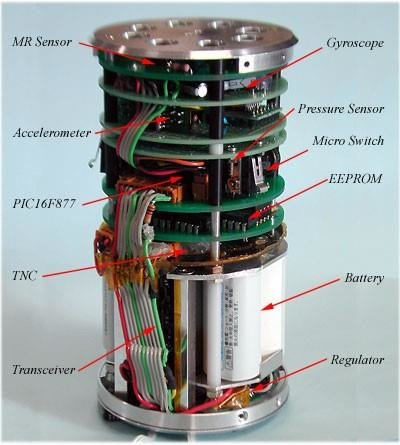
\includegraphics[width=0.5\textwidth]{Imagenes/Bitmap/cansat}
    \caption{Diagrama básico de un CanSat. Fuente: \cite{researchgate_cansat2018}}
    \label{fig:cansat}
\end{figure}


\section{Contexto}
El proyecto CanSat propuesto por el profesor Robert J. Twiggs en 1998~\cite{jaxa_cansat} comienza como un proyecto educativo basado en la simulación de un nanosatélite del tamaño de una lata de refresco y de un peso alrededor de los 350 gramos,
el objetivo es ayudar a los alumnos de distintos niveles a entender todas las fases de desarrollo de un satélite, desde la elección de la misión científica hasta la integración del sistema completo,
incluyendo los sensores necesarios para obtener los datos necesarios para dicha misión, la electronica necesaria para usar dichos sensores y enviarlos por radio a una estación de tierra,
la visualización de los datos, el diseño de una carcasa 3D capaz de aguantar la fuerza del lanzamiento y el diseño de un paracaídas.

Los CanSat no son puestos en órbita, pero son lanzados por cohetes a escala, globos aerostáticos o drones,
esto los somete a distintas fuerzas externas como aceleración, vibraciones o posibles impactos, lo que hace que el CanSat tenga que tener una estructura resistente.
La misión del CanSat es usar los sensores para recoger datos durante el descenso y transmitirlos a la estación de tierra.

Durante los últimos años la popularidad del proyecto ha ido aumentando, llegando a crear competiciones nacionales e internacionales lideradas por agencias espaciales como la agencia espacial europea~\cite{esa_cansat2024}
con el objetivo de promover el interés por el sector aeroespacial y por las carreras STEM en general desde pequeños.


\section{Motivación}
Debido a que estos proyectos suelen estar más enfocados en la parte electronica(recogida y transmisión de datos) y no tanto en la visualización de datos,
esta última parte suele quedar más descuidada, implementandose solo soluciones básicas como visualización de datos por consola o gráficas simples.
Además, estas soluciones son específicas para un CanSat concreto, lo que obliga a implementar soluciones desde cero.

Por ello, surge la necesidad de crear una plataforma común y reutilizable que permita visualizar en tiempo real los datos enviados por el CanSat y recibidos por la antena de manera más visual y profesional sin depender de un hardware concreto.
Con la creación de esta plataforma se facilitaría el análisis de los datos durante las pruebas y el lanzamiento,
además puede servir como base para futuras implementaciones específicas, ayudando a que los alumnos integren gráficas avanzadas sin tener que desarrollar una plataforma completa.


\section{Objetivos}
El objetivo principal de este proyecto consiste en diseñar y desarrollar desde cero un satélite tipo CanSat y la implementación una plataforma de visualización de datos reutilizable.
Para ello se han dividido los objetivos en dos partes diferenciadas: investigación de las tecnologías actuales y desarrollo del CanSat.

\begin{itemize}
    \item \textbf{Investigación}
    \begin{itemize}
        \item Comparación de los distintos microcontroladores y microcomputadores existentes para determinar cuál se ajusta mejor a los objetivos de nuestro desarrollo.
        \item Estudio de los distintos sensores disponibles en el mercado y su comunicación con el microcomputador.
        \item Análisis de las diferentes opciones de alimentación para el CanSat y de la posibilidad de cargarse con paneles solares.
        \item Comparación de las herramientas actuales de visualización de datos.
    \end{itemize}
    \item \textbf{Desarrollo}, dividido en dos partes: la creación del hardware del CanSat y la plataforma de visualización.
    \begin{itemize}
        \item CanSat
        \begin{itemize}
            \item Creación de un CanSat que cumpla con las medidas básicas (66mm x 115mm) y peso (entre 300g y 350g).
            \item Integración de receptor GPS
            \item Cámara para transmisión de video en tiempo real.
            \item Sensor de presión, temperatura y altitud.
            \item Giroscopio para obtener la orientación del dispositivo.
            \item Batería con posibilidad de carga mediante paneles solares.
            \item Retransmisión de los datos por WIFI si el dispositivo tiene conexión a internet.
            \item Retransmisión de los datos por radio en caso de que no tenga conexión.
            \item Desarrollo de un receptor de radio en la estación terrestre.
        \end{itemize}
        \item Plataforma de visualización
        \begin{itemize}
            \item Visualización en tiempo real de toda la telemetría recibida.
            \item Visualización del último valor de cada elemento de la telemetría.
            \item Gráficas en tiempo real de los valores recibidos.
            \item Visualización en tiempo real de las imágenes transmitidas.
            \item Mapa con la ubicación exacta del CanSat.
            \item Modelo 3D con la orientación real del CanSat.
            \item Descarga de los datos de telemetría para un rango de fechas concreto.
        \end{itemize}
    \end{itemize}
\end{itemize}


\section{Plan de trabajo}
Durante el desarrollo del proyecto se ha seguido un plan de trabajo con el objetivo de organizar las tareas y alcanzar los objetivos mencionados anteriormente.
Este plan de trabajo se ha dividido en los siguientes puntos:

\begin{itemize}
    \item Revisión y comparación de los microprocesadores Arduino y ESP32 y del microcomputador Raspberry Pi Zero 2 en función de sus capacidades y compatibilidad con los sensores y módulos de comunicación.
    \item Selección de los sensores (GPS, altímetro y giroscopio), módulo de comunicación (LoRa), cámara y sistema de alimentación.
    \item Ensamblaje inicial de los distintos componentes electrónicos usando placas de prototipado, lo que facilita las pruebas individuales de cada componente.
    \item Definición de la arquitectura general del sistema compuesta por tres componentes principales:
    \begin{itemize}
        \item Código embebido en la Raspberry Pi encargado de leer los sensores y transmisión de datos.
        \item Receptor de radio en tierra encargado de la recepción de los datos enviados por el CanSat.
        \item Plataforma de visualización en tiempo real.
    \end{itemize}
    \item Implementación del código embebido en la Raspberry usando Python y las distintas librerías para interactuar con cada sensor.
    \item Implementación de la plataforma de visualización en tiempo real basada en eventos, usando un sistema de colas RabbitMQ, un backend en Java y Spring Boot, un frontend en Flutter y una base de datos PostgreSQL para guardar los datos de telemetría.
    \item Soldar los componentes electrónicos en una placa definitiva de un tamaño que cumpla con las medidas reglamentarias de CanSat.
    \item Realización de pruebas de integración una vez todo el sistema esté terminando, incluyendo pruebas de duración de batería y de alcance de comunicaciones por radio.
    \item Redacción de la memoria documentando los pasos seguidos en el proyecto y los resultados obtenidos.
\end{itemize}


\section{Código fuente y licencia}

Todo el código desarrollado para este proyecto se encuentra disponible en un único repositorio público bajo la licencia MIT.

Incluye el backend, frontend y los scripts embebidos tanto en el CanSat como en la estación de tierra.

El repositorio está alojado en GitHub:

\url{https://github.com/tronxi/real-time-tracking-system}


\section{Organización de la memoria}

La memoria se compone de los siguientes capítulos:

\begin{itemize}
    \item \textbf{Capítulo 1. Introducción:} se presenta el contexto del proyecto, la motivación personal y académica, los objetivos planteados y el plan de trabajo seguido.

    \item \textbf{Capítulo 2. Trabajo relacionado:} se revisan iniciativas previas relacionadas con el concepto CanSat, tanto en el ámbito educativo como técnico, y se analizan distintas soluciones de adquisición, transmisión y visualización de datos.

    \item \textbf{Capítulo 3. Fundamentos teóricos:} se definen los conceptos técnicos necesarios para el desarrollo del sistema, incluyendo comparativas de hardware, tecnologías de comunicación, sensores, protocolos de vídeo y arquitecturas de visualización en tiempo real.

    \item \textbf{Capítulo 4. Diseño e implementación del sistema:} se describe la arquitectura del sistema completo, los componentes elegidos, el montaje del CanSat, el desarrollo del software embebido, el backend, el frontend y las pruebas realizadas.

    \item \textbf{Capítulo 5. Conclusiones y trabajo futuro:} se recogen las principales conclusiones del trabajo, se valoran los resultados obtenidos y se proponen posibles mejoras y líneas de desarrollo futuras.
\end{itemize}
\chapter{Trabajo relacionado}
\label{cap:trabajorRelacionado}
En este capítulo vamos a contextualizar el concepto CanSat y se revisarán trabajos relacionados con este tipo de sistemas.
Primero se describirá en detalle que es un CanSat y las principales iniciativas educativas que los promueven,
algunas competiciones educativas y normativa para participar.
A continuación, se presentarán las soluciones más habituales de adquisición y transmisión de datos, así como las herramientas existentes para visualización de telemetría en tiempo real.


\section{Proyectos educativos y competiciones CanSat}
Desde su creación en 1998 por Robert J. Twiggs, el concepto CanSat ha sido muy utilizado para referirse a satélites suborbitales de bajo coste,
ligeros y de tamaño contenido.
El objetivo de estos satélites está mayormente asociado al ámbito educativo, donde se usan para dar una introducción a los estudiantes al desarrollo real de una misión espacial,
teniendo en cuenta todas las fases de una misión científica real, definición de los objetivos científicos, elección de los componentes, diseño de la arquitectura, ensamblaje de los componentes,
diseño de la estación de tierra y visualización y procesado de los datos.

En la actualidad, varias instituciones y agencias espaciales realizan competiciones anuales dirigidas a estudiantes de todas las edades para desarrollar sus propios CanSat.
Estas competiciones se basan en lanzar el CanSat con un cohete a escala, desde un drone o globo aerostático y recibir datos durante el tiempo de descenso.

Algunas de estas competiciones son la \cite{cansatcompetition2025}, organizada por la \cite{american_astronautical_society2025} dirigida a estudiantes universitarios
y \cite{esa_cansat2025} organizada por la \cite{esa2025} y dirigida a grupos de estudiantes de entre 14 y 19 años.
Esta competición organiza torneos regionales y una final a nivel europeo con los mejores representantes de cada país.

\begin{figure}
    \centering
    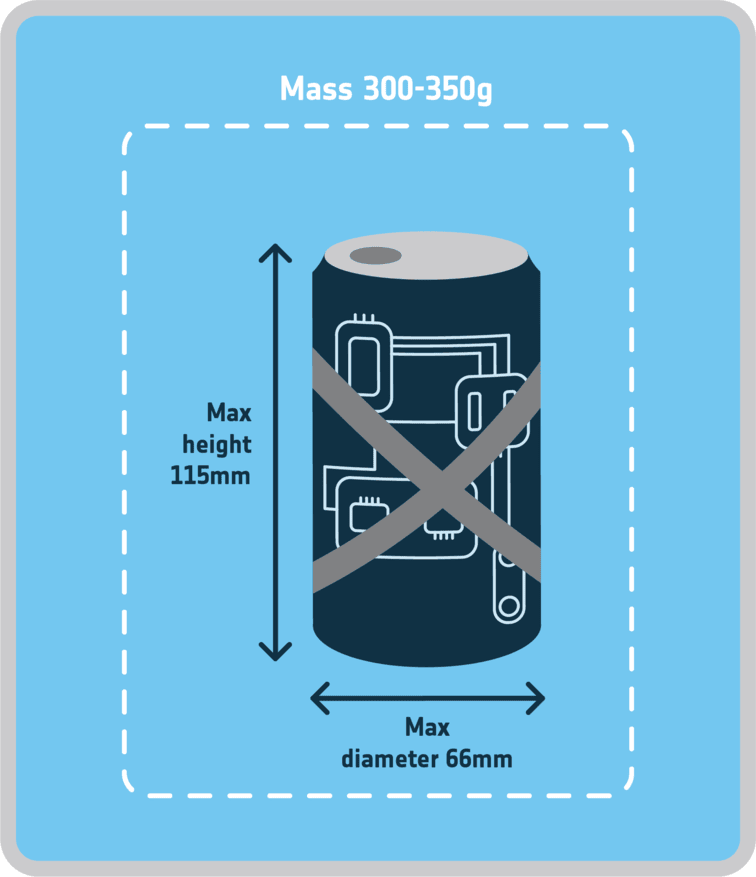
\includegraphics[width=0.4\textwidth]{Imagenes/Bitmap/cansat_size}
    \caption{Medidas máximas de un CanSat para una competición europea}
    \label{fig:cansat_Size}
\end{figure}

Los requisitos que debe cumplir un CanSat para participar en una competición europea son:
\begin{itemize}
    \item Deben tener una altura máxima de 115mm y un diámetro máximo de 66mm.
    \item Un peso entre 300 y 350 gramos.
    \item Deben cumplir una misión principal basada en medir la presión y temperatura del aire y enviarlo a la estación de tierra al menos una vez por segundo.
    \item Una misión secundaria elegida por cada equipo.
    \item No deben incluir materiales inflamables, explosivos o peligrosos para el medio ambiente.
    \item Debe estar alimentado por batería o paneles solares que lo mantengan encendido durante al menos cuatro horas.
    \item La batería debe ser accesible y fácil de reemplazar o cargar.
    \item Incluir un interruptor de encendido y apagado accesible.
    \item Incluir un paracaídas que facilite la recuperación del CanSat después del lanzamiento y que garantice un tiempo de vuelo máximo de 120 segundos.
    \item El ratio de descenso debe estar entre 8 y 11m/s.
    \item Soportar una aceleración de hasta 20g.
    \item El coste total del CanSat no puede superar los 500€.
\end{itemize}


\section{Sistemas de adquisición y transmisión de datos para CanSat}
Los sistemas de adquisición y transmisión de datos utilizados en los CanSat siguen una arquitectura similar a la empleada en las misiones espaciales reales.
Esta arquitectura se basa en dos flujos de comunicación realizados entre el satélite y la estación de tierra:
\begin{itemize}
    \item \textbf{Uplink:} Enviar telecomandos al satélite desde tierra, en el caso de los CanSat esto es poco común.
    \item \textbf{Downlink:} Recibir telemetría desde el satélite a la estación de tierra.
\end{itemize}

\begin{figure}
    \centering
    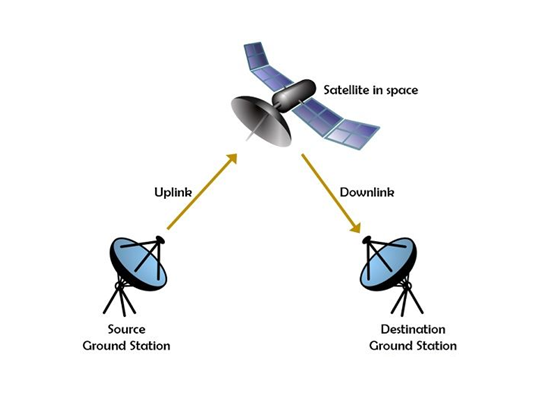
\includegraphics[width=0.8\textwidth]{Imagenes/Bitmap/upling_downlink}
    \caption{Ejemplo de comunicación Uplink/Downlink}
    \label{fig:uplink_downlink}
\end{figure}

Para llevar a cabo esta comunicación, los CanSat deben incluir una serie de componentes básicos:
\begin{itemize}
    \item \textbf{Ordenador a bordo (OBC, On-Board Computer):} Encargado de la comunicación con los sensores y el módulo de transmisión, Puede estar basado en microcontroladores (como Arduino o ESP32) o microcomputadores (como Raspberry Pi).
    \item \textbf{Módulo de comunicación:} se encarga de la transmisión de datos mediante tecnologías como LoRa \cite{lora2015overview}, XBee \cite{xbee} o Wi-Fi, dependiendo del alcance necesario,
    la elección de la frecuencia de transmisión depende tanto del módulo que se utilice como de la normativa de cada país, además, debe poderse cambiar con facilidad para no interferir con otros CanSat.
    \item \textbf{Sensores:} permiten adquirir información relevante sobre el entorno, como presión atmosférica, temperatura, orientación (IMU) o localización geográfica (GPS).
    \item \textbf{Fuente de alimentación:} normalmente una batería recargable, capaz de mantener operativo el sistema durante toda la misión. En algunos casos puede complementarse con pequeños paneles solares.
\end{itemize}

Estos componentes forman la base mínima que un CanSat necesita para poder llevar a cabo la misión científica y comunicar los datos con la estación de tierra.


\section{Soluciones existentes para telemetría y visualización de datos}
Normalmente, los proyectos CanSat están más enfocados en el diseño electrónico y la comunicación por radio,
por lo que se suele desarrollar menos la parte de visualización de datos, utilizando por lo general herramientas genéricas
o limitadas al ordenador en el que está corriendo la estación de tierra, algunas de estas herramientas son:

\begin{itemize}
    \item \textbf{\cite{serialplot}}:herramienta ligera que permite graficar en tiempo real los datos recibidos por puerto serie.
    Es muy usada durante el desarrollo por su sencillez y rapidez para validar sensores, aunque no permite guardar datos ni personalizar la interfaz.
    \item \textbf{Matplotlib}~\cite{matplotlib}, ~\textbf{\cite{pyqtgraph}} o~\textbf{\cite{tkinter}}: librerías desarrolladas en python, permiten construir interfaces personalizadas, pero no están pensadas para ser accesibles a través de una interfaz web y requieren conocimientos de programación hasta para los casos más simples.
    \item \textbf{\cite{excel}} o~\textbf{\cite{googlesheets}}: se utilizan exportando directamente los datos recibidos, no requieren conocimientos de programación pero no permiten la visualización en tiempo real.
    \item \textbf{\cite{labview}} entorno gráfico profesional diseñado para adquisición y visualización de datos en sistemas embebidos e instrumentación industrial.
    Permite construir interfaces complejas mediante programación visual y cuenta con soporte nativo para muchos dispositivos de hardware.
    Aunque es muy potente, tiene un coste elevado de licencia y una curva de aprendizaje considerable, por lo que raramente se utiliza en proyectos educativos como CanSat.
\end{itemize}

En resumen, la gran mayoría de herramientas son o muy básicas o demasiado potentes para el uso necesario en un CanSat, además ninguna de estas es específica para el tipo de datos y gráficos habituales en este tipo de proyectos.

\chapter{Fundamentos teóricos}
\label{cap:fundamentos_teoricos}
\section{Comparativa de microcontroladores: Arduino, ESP32 y Raspberry Pi Zero 2}
\section{Protocolos de comunicación: I2C y UART}
\section{Transmisión de datos mediante LoRa}
\section{Sensores embarcados: presión, orientación y GPS}
\section{Captura y transmisión de vídeo en tiempo real}
\section{Visualización de datos en tiempo real: arquitecturas orientadas a eventos}
\section{Modelado 3D de orientación con cuaterniones}
\chapter{Diseño e implementación del sistema}
Este capítulo describe la arquitectura general del sistema y detalla cada uno de sus componentes, desde el montaje electrónico del CanSat hasta la visualización de los datos en tiempo real.

Se justifica la elección del hardware y software empleados, se explica el funcionamiento del código embebido, y se documenta la integración entre los distintos módulos del sistema: la Raspberry Pi, el backend en Spring Boot, la base de datos, el broker de eventos RabbitMQ y el frontend desarrollado en Flutter.

Finalmente, se presentan las pruebas realizadas para verificar el funcionamiento del sistema completo.


\section{Selección de componentes y tecnologías utilizadas}


Este apartado describe los principales elementos hardware y software empleados en el sistema.

La selección se ha basado en los requisitos técnicos del proyecto y en las conclusiones del análisis comparativo desarrollado en el capítulo anterior.

\begin{itemize}
    \item \textbf{Unidad de procesamiento:} se ha utilizado una~\cite{raspberrypi_zero2}.

    \begin{figure}[H]
        \centering
        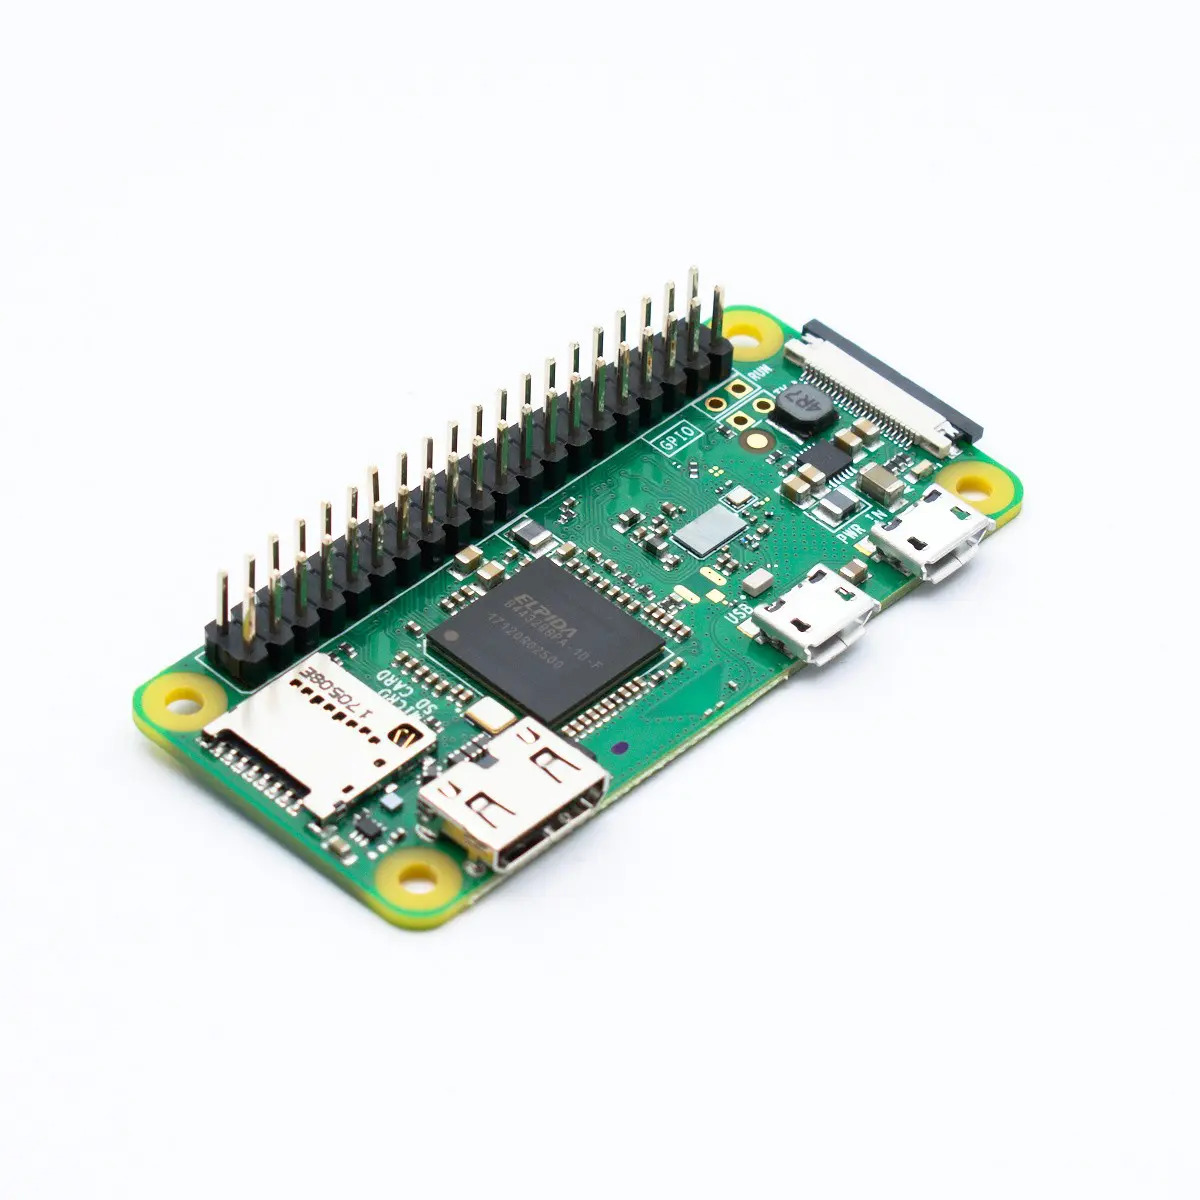
\includegraphics[width=0.2\textwidth]{Imagenes/Bitmap/ras2}
        \caption{Raspberry Pi Zero 2 W}
        \label{fig:ras2}
    \end{figure}

    Su capacidad para ejecutar Linux, capturar y codificar vídeo por hardware, y gestionar interfaces como I\textsuperscript{2}C, UART y CSI, la hacen adecuada para su integración directa en un CanSat sin necesidad de microcontroladores adicionales.
    \item \textbf{Sensor de presión barométrica:} el BMP388~\cite{adafruitBMP388} permite estimar la altitud mediante medición barométrica.
    Además de la presión atmosférica, proporciona la temperatura del entorno.
    Ofrece una precisión de ±8~Pa, bajo consumo y comunicación por I\textsuperscript{2}C.

    \begin{figure}[H]
        \centering
        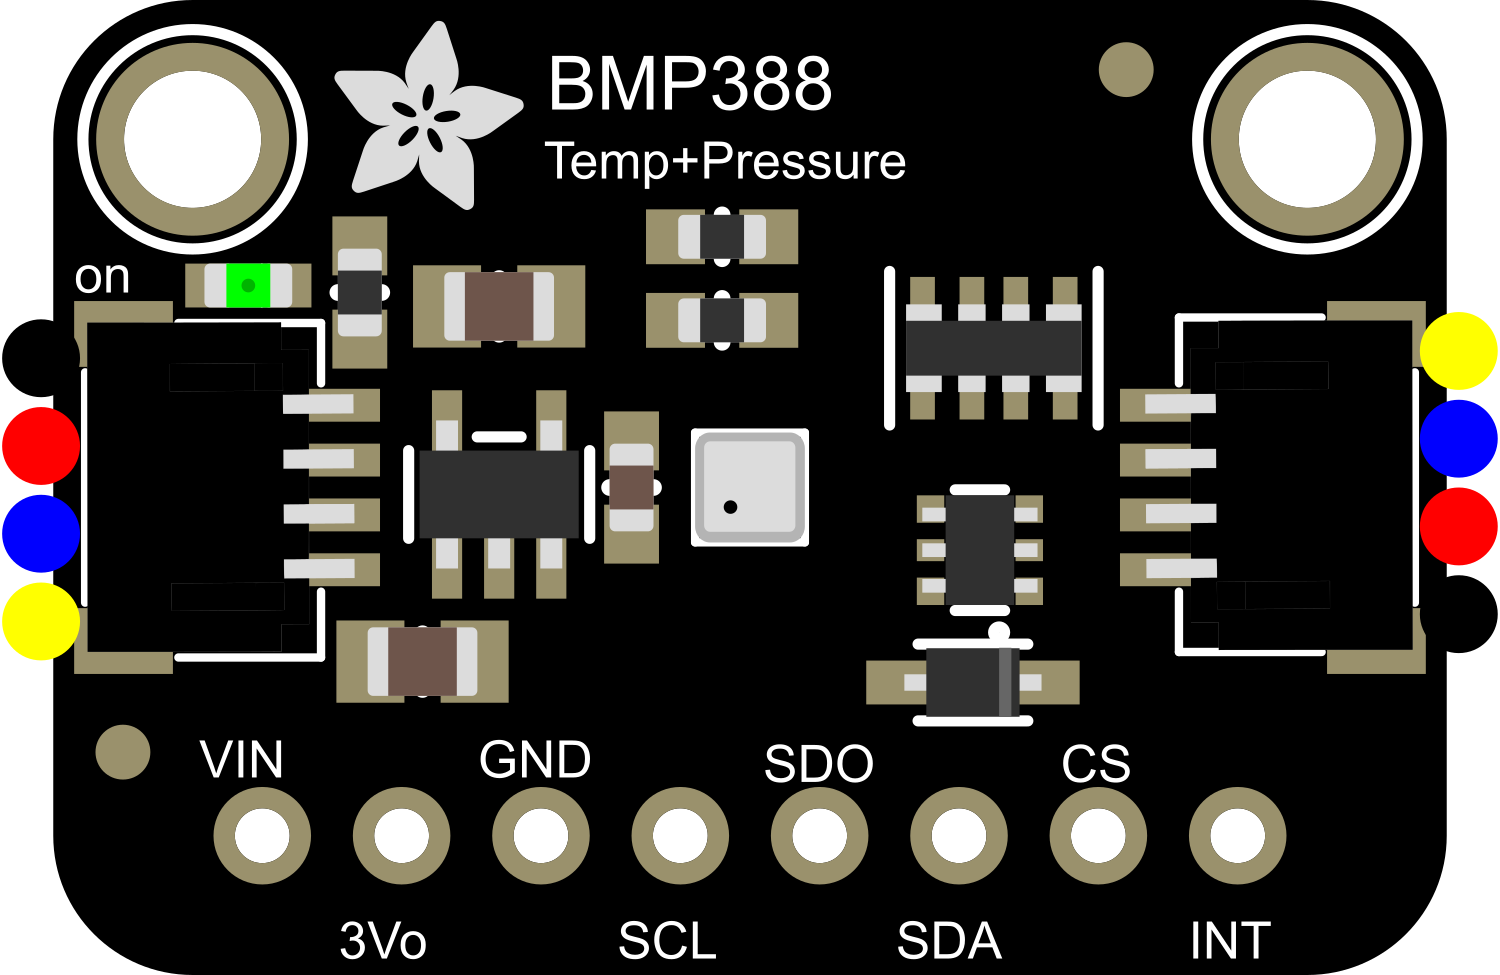
\includegraphics[width=0.4\textwidth]{Imagenes/Bitmap/bmp388}
        \caption{Sensor de presión barométrica bmp388}
        \label{fig:bmp388}
    \end{figure}

    \item \textbf{IMU:} Se ha empleado el BNO085~\cite{adafruitBNO085}, un sensor de 9 grados de libertad que combina acelerómetro, giroscopio y magnetómetro.
    Incorpora un procesador dedicado que realiza la fusión sensorial internamente y entrega directamente la orientación absoluta, lo que evita cálculos adicionales en la Raspberry Pi.

    \begin{figure}[H]
        \centering
        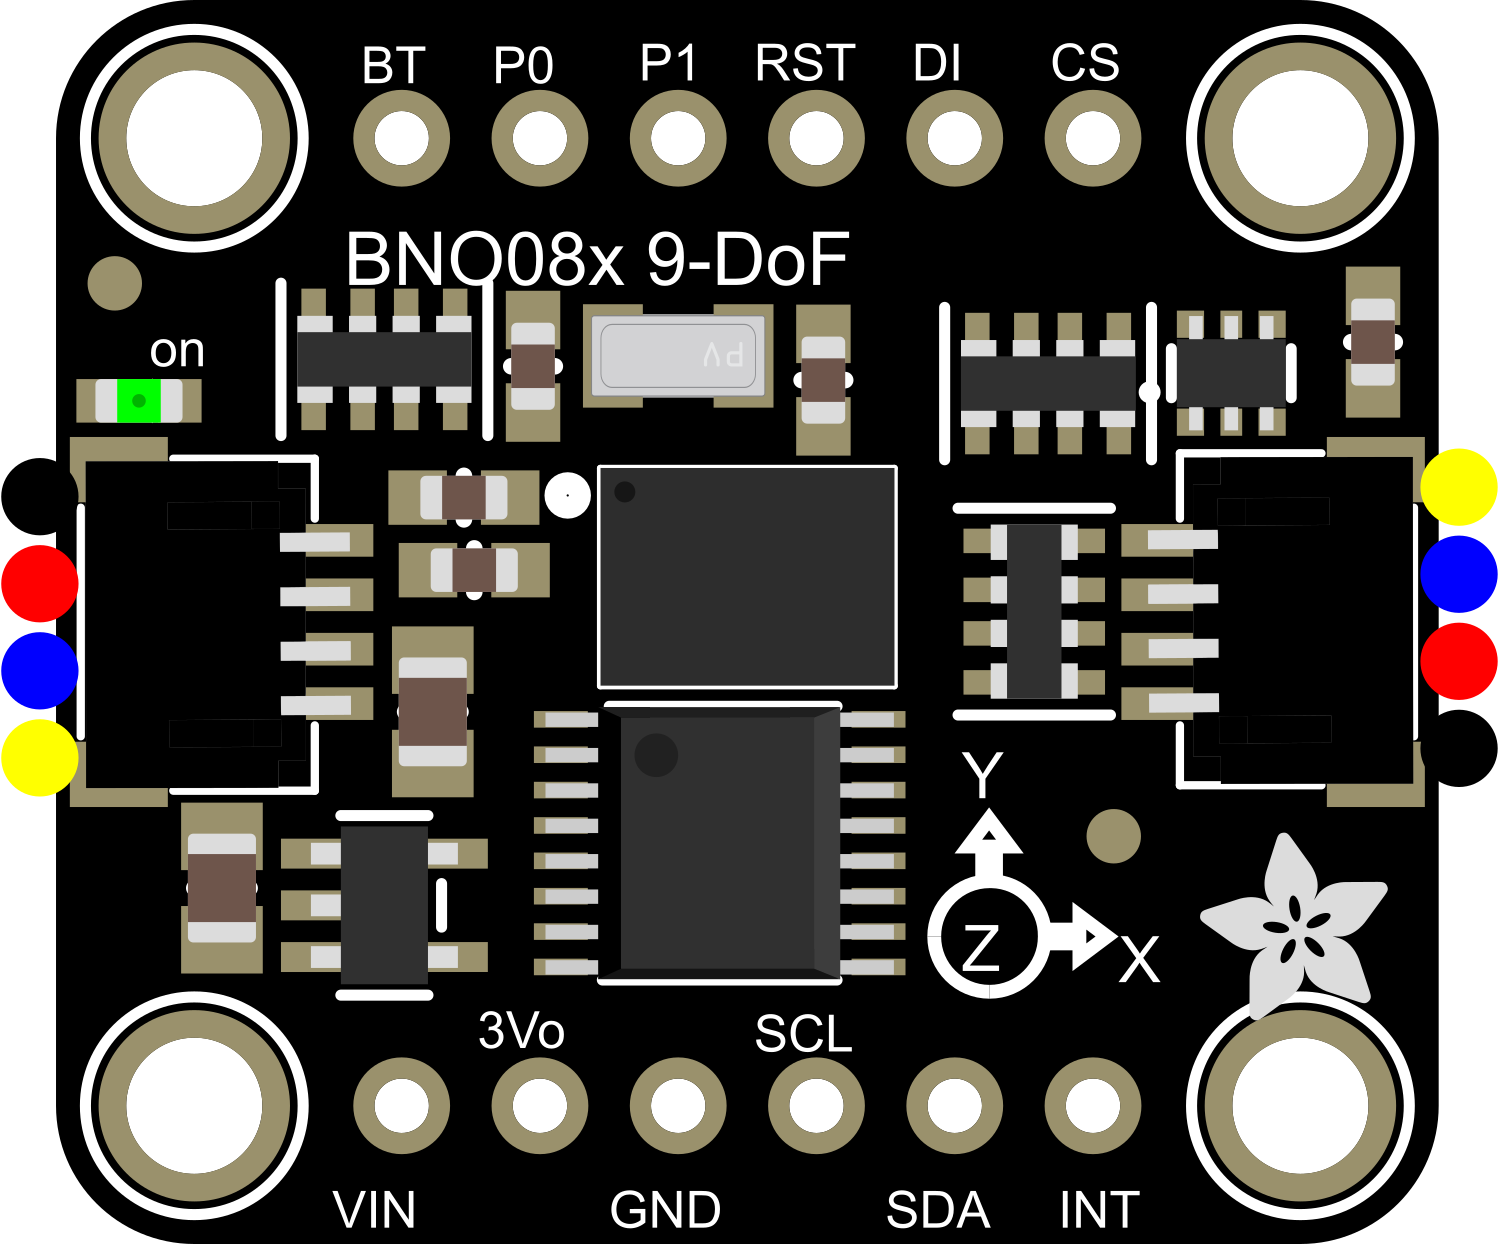
\includegraphics[width=0.4\textwidth]{Imagenes/Bitmap/bno085}
        \caption{IMU bno085}
        \label{fig:bno085}
    \end{figure}
    \item \textbf{GNSS:} se ha utilizado el módulo BN-880~\cite{bn880Module}, que integra un receptor GNSS con soporte para múltiples constelaciones (GPS, GLONASS, Galileo y BeiDou).
    Proporciona datos de posición, velocidad y altitud en tiempo real mediante interfaz UART. Incluye una antena activa integrada y una brújula electrónica.
    \begin{figure}[H]
        \centering
        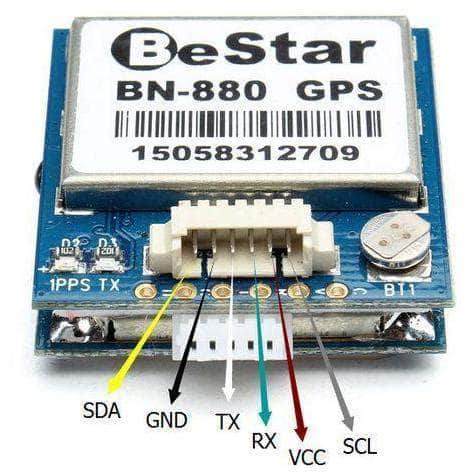
\includegraphics[width=0.4\textwidth]{Imagenes/Bitmap/bn-880}
        \caption{GPS bn-880}
        \label{fig:bn-880}
    \end{figure}
    \item \textbf{Cámara:} se utiliza el modelo oficial de la Raspberry Pi~\cite{raspiCamV2} con interfaz CSI. Permite la captura de vídeo codificado en H.264 mediante la GPU, sin comprometer el rendimiento del sistema.
    \begin{figure}[h]
        \centering
        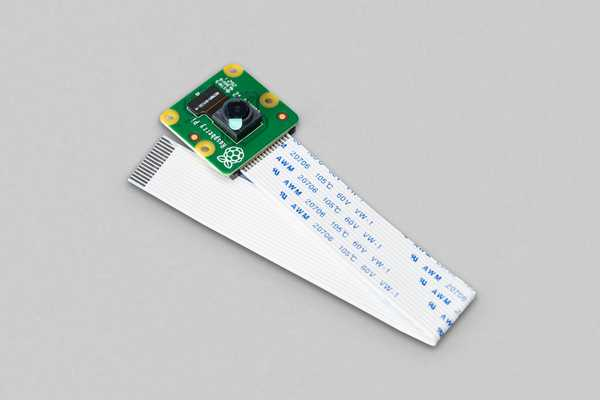
\includegraphics[width=0.4\textwidth]{Imagenes/Bitmap/rascamv2}
        \caption{Raspberry Pi Camera Module 2}
        \label{fig:rascamv2}
    \end{figure}
    \item \textbf{Transmisión de datos:} el sistema utiliza Wi-Fi si hay red disponible, en caso contrario el módulo LoRa E32-900T20D~\cite{ebyteE32}.
    Este módulo opera en 868~MHz y permite comunicación a larga distancia mediante UART.
    \begin{figure}[h]
        \centering
        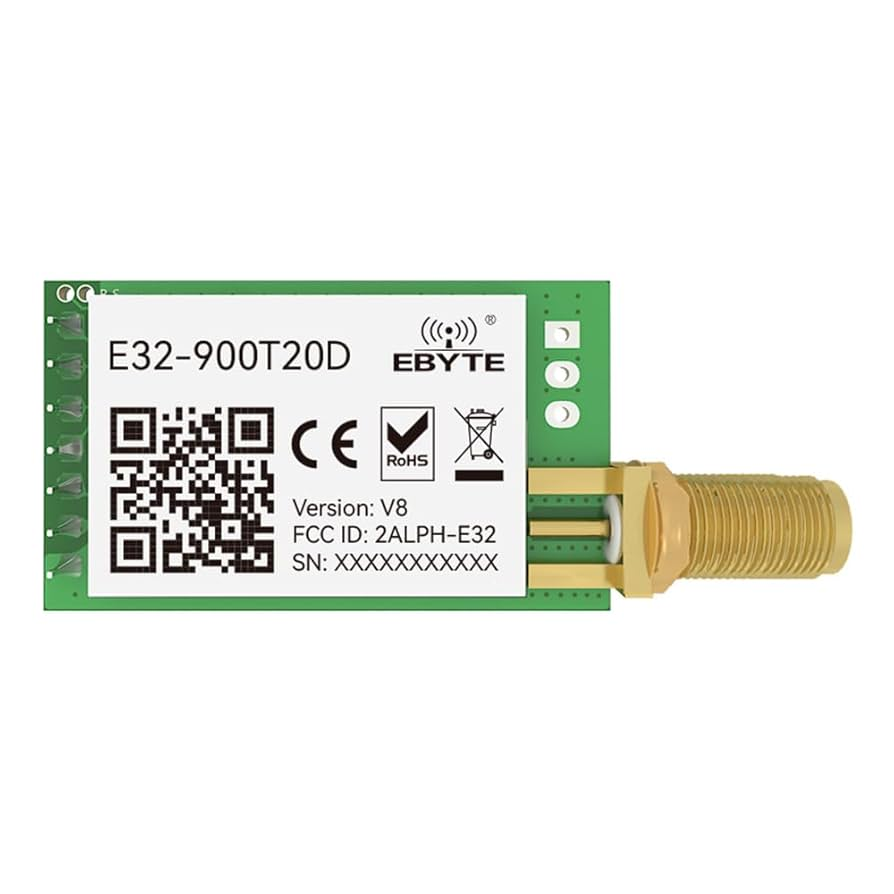
\includegraphics[width=0.4\textwidth]{Imagenes/Bitmap/lorae32}
        \caption{Módulo LoRa E32-900T20D}
        \label{fig:lorae32}
    \end{figure}

    \item \textbf{Antena LoRa:} se utiliza una antena externa de 868–915~MHz, con conector SMA macho, ganancia de 3~dBi e impedancia de 50~\(\Omega\).

    \begin{figure}[h]
        \centering
        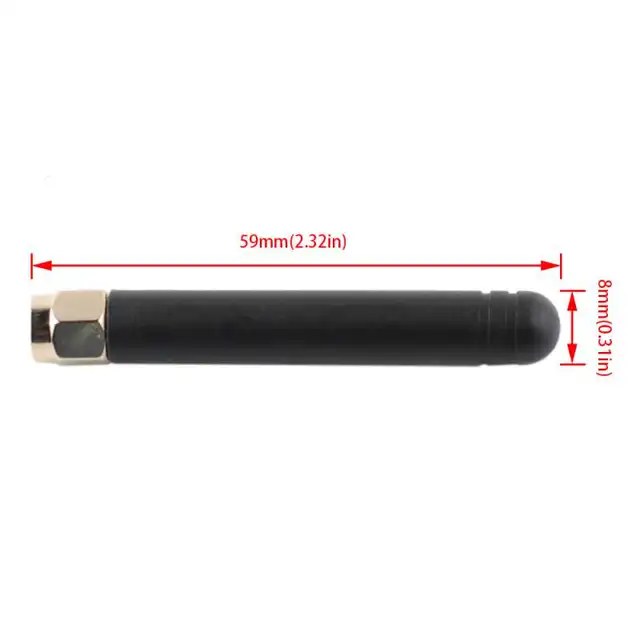
\includegraphics[width=0.4\textwidth]{Imagenes/Bitmap/antena_lora}
        \caption{Antena LoRa U.FL a SMA 868–915~MHz, 3~dBi}
        \label{fig:antena_lora}
    \end{figure}

    \item \textbf{Alimentación:} el sistema se alimenta mediante una batería recargable de ion de litio (Li-ion) tipo 18650 de 3{,}7~V conectada a un cargador MCP73871~\cite{mcp73871Datasheet}, que permite la recarga mediante panel solar y proporciona protección frente a sobrecarga, descarga profunda y cortocircuitos.

    Para obtener los 5~V requeridos por la Raspberry Pi, se emplea un convertidor elevador DC-DC ajustable (modelo VISSQH), que incrementa la tensión de entrada hasta una salida estabilizada.

    \begin{figure}[H]
        \centering
        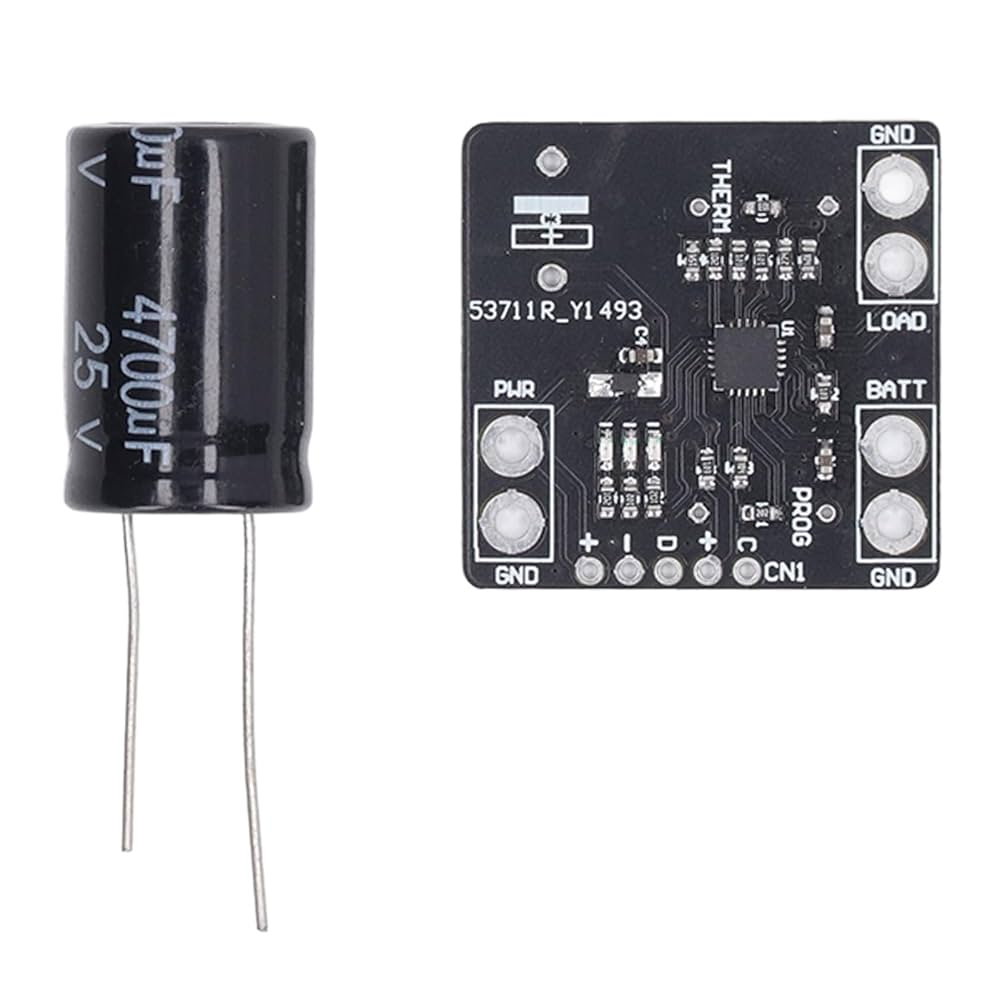
\includegraphics[width=0.4\textwidth]{Imagenes/Bitmap/mcp73871}
        \caption{Cargador MCP73871}
        \label{fig:mcp73871}
    \end{figure}
    \begin{figure}[H]
        \centering
        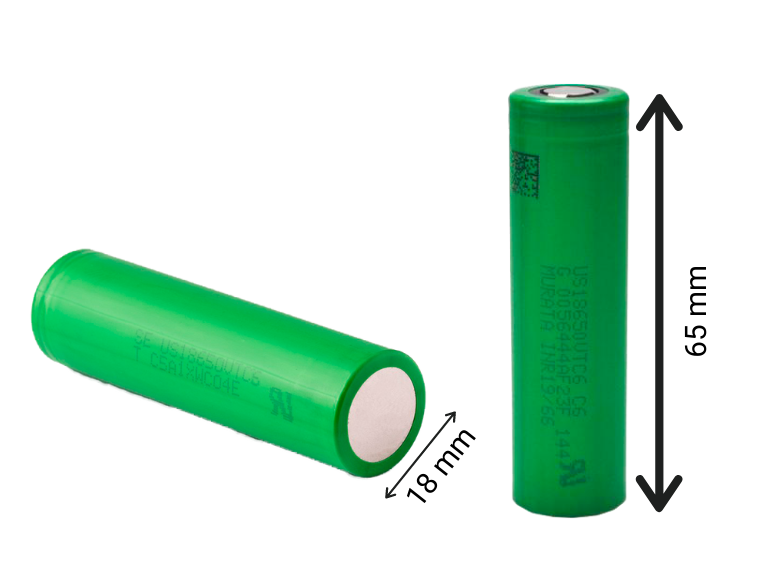
\includegraphics[width=0.4\textwidth]{Imagenes/Bitmap/18650}
        \caption{Batería 18650}
        \label{fig:18650}
    \end{figure}
    \item \textbf{Estación de tierra:} está formada por un receptor LoRa conectado mediante UART a una Raspberry Pi 4.

    Esta actúa como pasarela entre el CanSat y el sistema de mensajería RabbitMQ, reenviando los datos recibidos a través de LoRa.

    \item \textbf{Software embebido:} tanto la Raspberry Pi usada en el CanSat como la de la estación de tierra ejecutan scripts desarrollados en Python.

    \item \textbf{Software del sistema:} el backend está desarrollado en Java utilizando el framework Spring Boot, que facilita la construcción de servicios web REST y la integración con sistemas de mensajería.

    Para el intercambio de mensajes se emplea RabbitMQ, un sistema de colas que implementa el protocolo AMQP.

    La persistencia de datos se gestiona con PostgreSQL, un sistema de gestión de bases de datos relacional.

    La interfaz de usuario está implementada en Flutter, un framework multiplataforma desarrollado en Dart, y establece la comunicación en tiempo real mediante WebSocket utilizando el protocolo STOMP.
\end{itemize}


\section{Arquitectura general del sistema}
La arquitectura del sistema se organiza en tres bloques principales: el CanSat, la estación de tierra y la infraestructura de backend y visualización web.

Esta arquitectura sigue un enfoque orientado a eventos, en el que los datos generados por el CanSat son publicados y transmitidos hacia los consumidores mediante mecanismos de mensajería asincrónica.

Los tres componentes principales son:

\begin{itemize}
    \item \textbf{CanSat: }integra sensores, módulo GNSS, cámara y comunicaciones.

    Una Raspberry Pi Zero 2 W adquiere y empaqueta los datos de telemetría para su envío.
    Cuando hay red Wi‑Fi disponible, los eventos se publican directamente en un broker RabbitMQ. En caso contrario, los datos se transmiten mediante LoRa a la estación de tierra.

    Todos los datos de telemetría adquiridos por los sensores se guardan de manera local en formato JSON.
    En cuanto a la retransmisión de vídeo en tiempo real, solo se realiza cuando está conectado a una red Wi-Fi, en caso contrario, el vídeo se guarda en la memoria de la Raspberry Pi.

    \item \textbf{Estación de tierra: }compuesta por una Raspberry Pi 4 conectada al receptor LoRa mediante UART.

    Ejecuta un script en Python que interpreta los paquetes recibidos y los reenvía al broker RabbitMQ a través de la red.

    Esta estación actúa como pasarela cuando no hay conectividad directa entre el CanSat y la infraestructura de backend en los casos en los que no existe conexión directa mediante red.

    \item \textbf{Infraestructura de visualización: } esta infraestructura está formada por varios componentes:
    \begin{itemize}
        \item \textbf{RabbitMQ: } recibe los eventos de telemetría desde la estación de tierra o directamente desde el CanSat y los transmite al backend.
        \item \textbf{Backend: } se encarga de consumir los eventos con los datos de telemetría que llegan desde RabbitMQ,
        guardarlos en la base de datos para su posterior descarga, y emitir los eventos hasta el frontend utilizando websockets.
        \item \textbf{Base de datos: } se trata de una base de datos relacional PostgreSQL, en ella se guardan todos los eventos de telemetría asociados a su fecha de recepción.
        \item \textbf{Frontend: } es una aplicación web desarrollada en Flutter, cuenta con distintos tipos de gráficas para visualizar los datos del CanSat en tiempo real a través de WebSockets.
        \item \textbf{Servidor de vídeo en tiempo real:} recibe el flujo de vídeo codificado desde el CanSat mediante el protocolo RTMP y lo adapta para su reproducción en navegadores web.
        La transmisión solo se realiza cuando hay conectividad Wi‑Fi disponible.
    \end{itemize}
    Para mejorar la portabilidad y facilitar el despliegue de la infraestructura en distintos entornos, todos los servicios del backend, la base de datos, el broker de mensajería y el servidor de vídeo se han contenerizado utilizando Docker.
\end{itemize}
\begin{figure}[H]
    \centering
    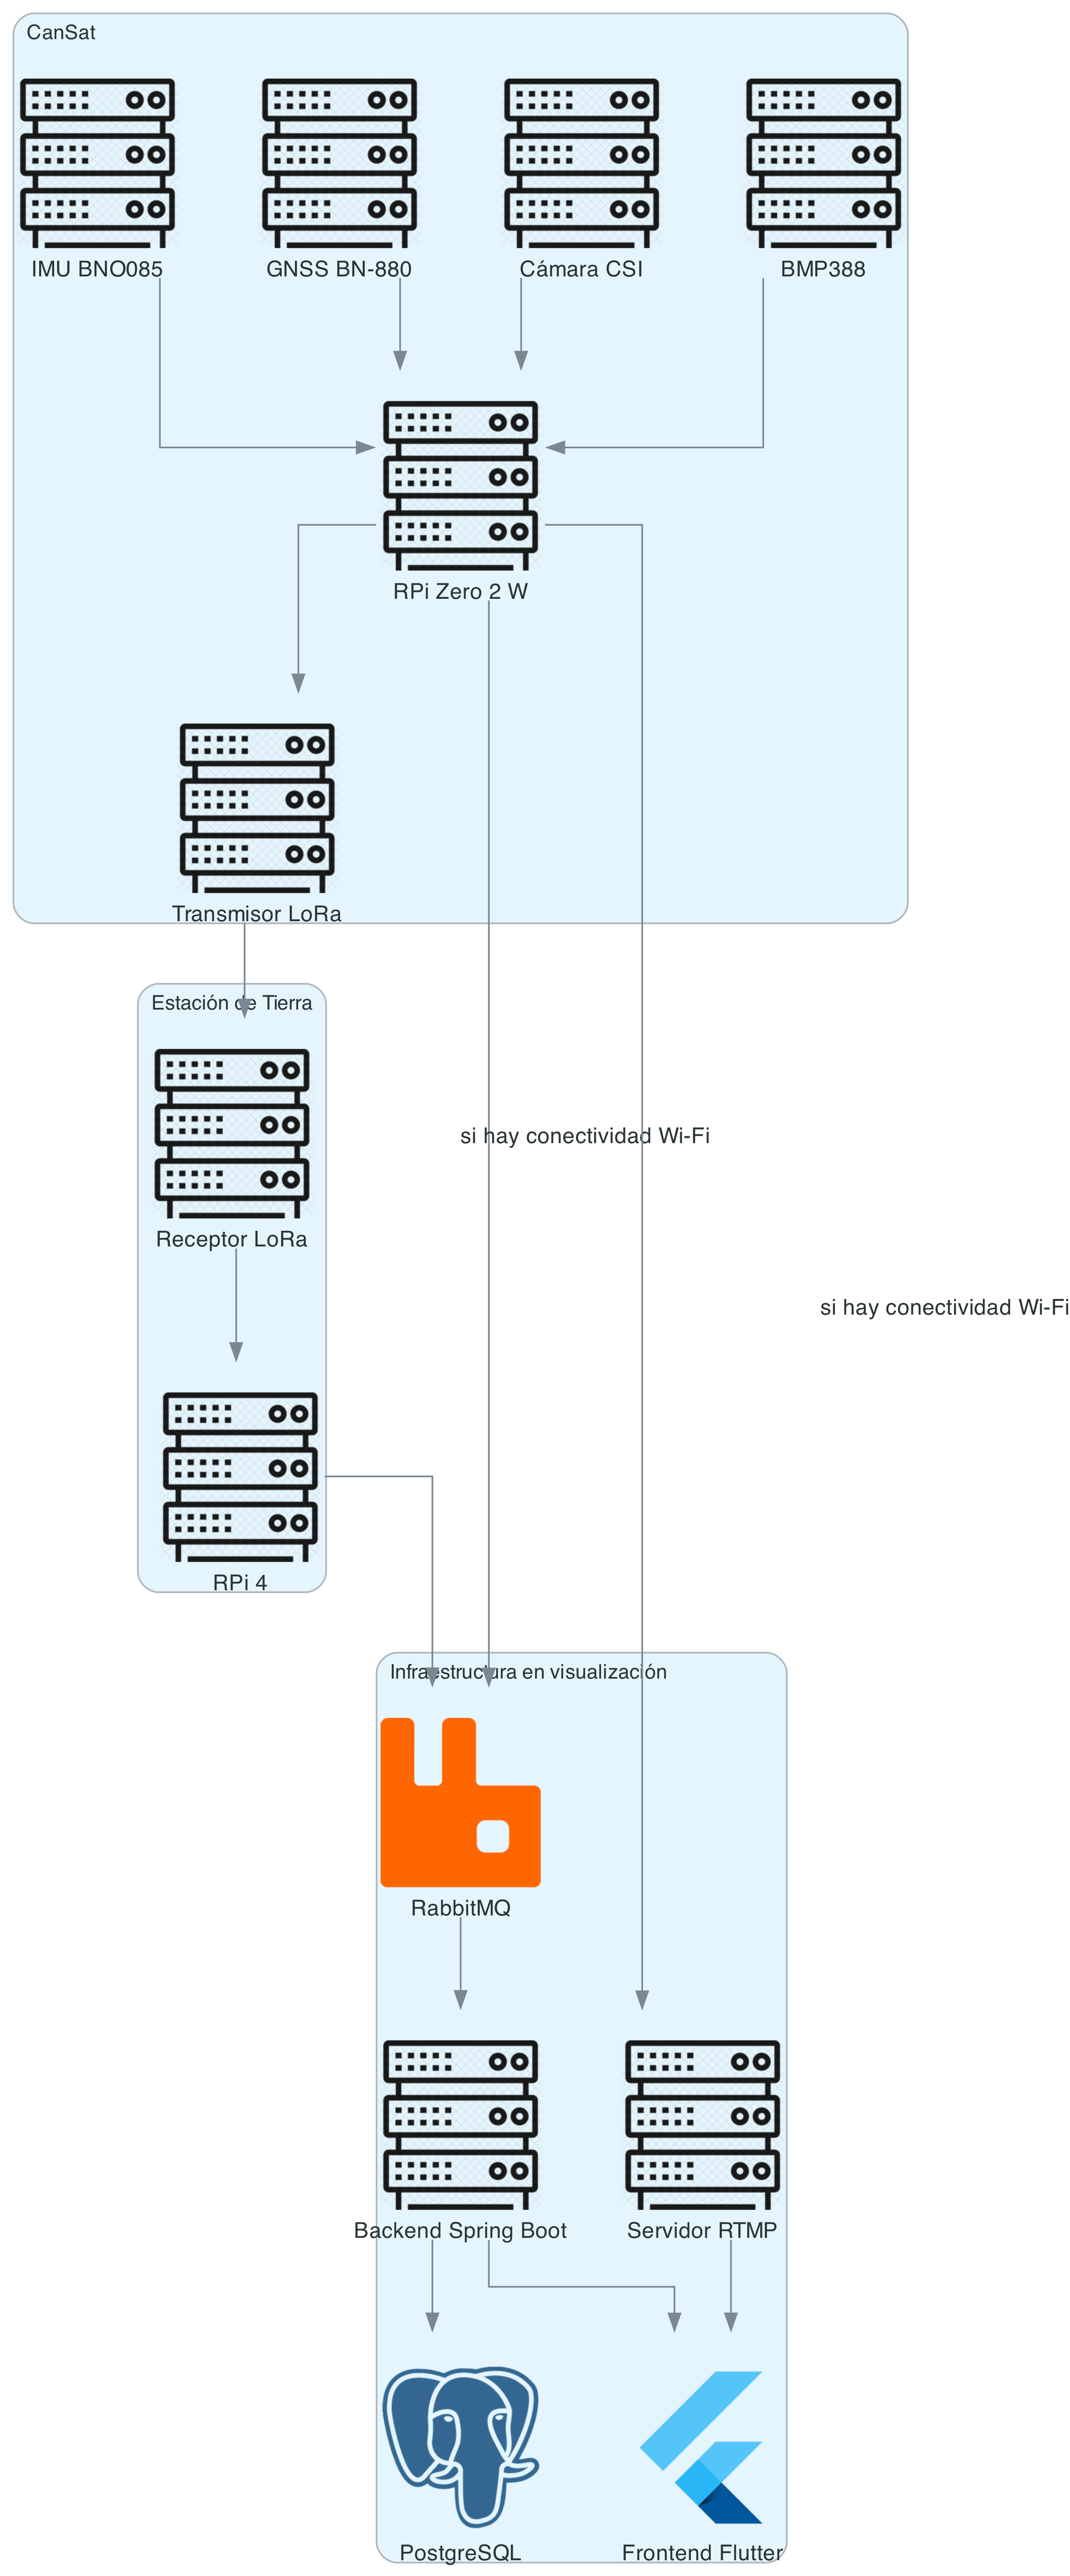
\includegraphics[width=0.51\textwidth]{Imagenes/Bitmap/cansat_architecture}
    \caption{Arquitectura general del sistema}
    \label{fig:cansat_architecture}
\end{figure}


\section{Montaje electrónico del CanSat}
El montaje electrónico se realizó inicialmente sobre una protoboard, con el objetivo de validar las conexiones y el funcionamiento de los distintos módulos durante la fase de desarrollo.

Cada componente fue integrado mediante cableado directo a la Raspberry Pi Zero 2 W, usando las interfaces específicas de cada uno (UART, I\textsuperscript{2}C).

A continuación, se describen las conexiones realizadas entre los distintos periféricos y la Raspberry Pi, incluyendo los pines utilizados y las interfaces empleadas.

\begin{itemize}
    \item \textbf{Sensor de presión BMP388:} utiliza la interfaz I\textsuperscript{2}C.
    \begin{itemize}
        \item SDA: GPIO~2 (pin físico~3)
        \item SCL: GPIO~3 (pin físico~5)
        \item Alimentación: 5~V (pin físico~2)
        \item GND: pin físico~6
    \end{itemize}

    \item \textbf{IMU BNO085:} también conectada por I\textsuperscript{2}C en el mismo bus que el BMP388.
    \begin{itemize}
        \item SDA: GPIO~2 (pin físico~3)
        \item SCL: GPIO~3 (pin físico~5)
        \item Alimentación: 5~V (pin físico~2)
        \item GND: pin físico~6
    \end{itemize}

    \item \textbf{Módulo LoRa E32-900T20D:} comunica por UART.
    \begin{itemize}
        \item TX del módulo → RX de la Pi: GPIO~15 (pin físico~10)
        \item RX del módulo ← TX de la Pi: GPIO~14 (pin físico~8)
        \item Alimentación: 5~V (pin físico~2)
        \item GND: pin físico~6
        \item Pines M0 y M1: conectados respectivamente a los GPIO~23 (pin físico~16) y GPIO~24 (pin físico~18) de la Raspberry Pi, lo que permite gestionar el modo de operación del módulo desde software.
        \item Conexión de antena: la antena externa se conecta al conector SMA hembra del módulo LoRa, permitiendo la comunicación en la banda de 868–915~MHz.
    \end{itemize}
    \begin{figure}[H]
        \centering
        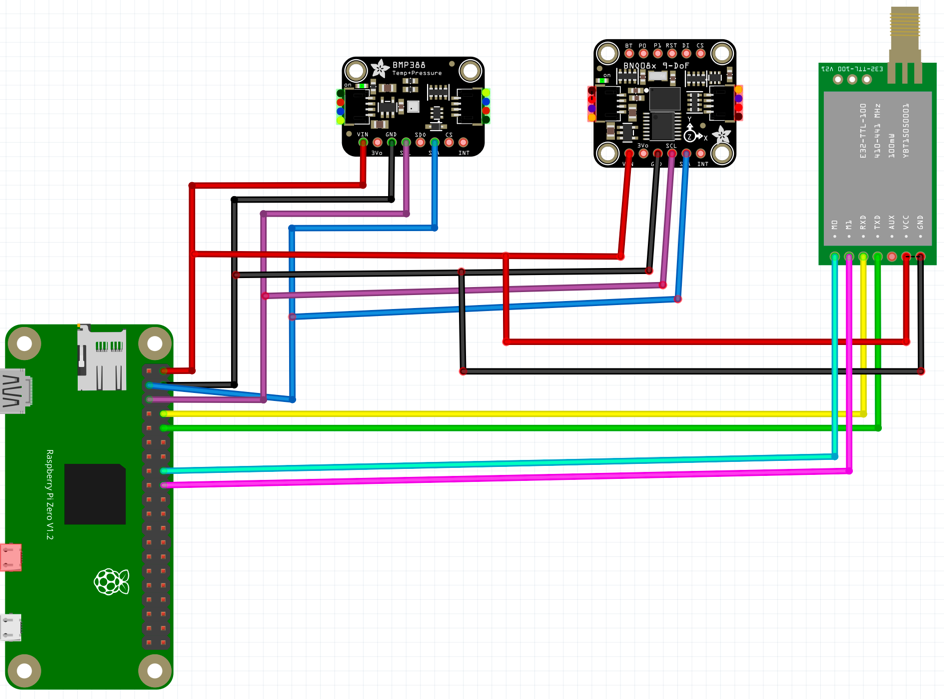
\includegraphics[width=0.7\textwidth]{Imagenes/Bitmap/conexion_sensores}
        \caption{Diagrama de conexión de los sensores y módulo LoRa}
        \label{fig:conexion_sensores}
    \end{figure}
    \item \textbf{GNSS BN-880:} comunica por UART. Dado que la Raspberry Pi Zero 2~W solo dispone de un puerto UART hardware accesible por GPIO (usado en este caso por el módulo LoRa),
    se ha optado por conectar el BN-880 a través de un adaptador USB a UART.

    El módulo utilizado es un conversor basado en el chip CP2102, que se conecta al puerto micro-USB de la Raspberry Pi y proporciona una interfaz UART adicional accesible desde el sistema operativo como un puerto /dev/ttyUSB0.

    Dado el espacio reducido disponible, se ha modificado el adaptador CP2102 retirando el conector USB macho original y sustituyéndolo por un conector micro-USB macho, soldado directamente a la placa.
    Esto permite conectarlo al puerto micro-USB de datos de la Raspberry Pi de forma más compacta, sin necesidad de adaptadores adicionales.

    \begin{itemize}
        \item TX del GNSS → RX del adaptador
        \item RX del GNSS ← TX del adaptador
        \item Alimentación: 5~V conectado al pin VCC del adaptador
        \item GND: pin físico~14 conectado al GND del adaptador
        \item Conexión de datos: vía micro-USB del adaptador al puerto USB de la Raspberry Pi
    \end{itemize}
    \begin{figure}[H]
        \centering
        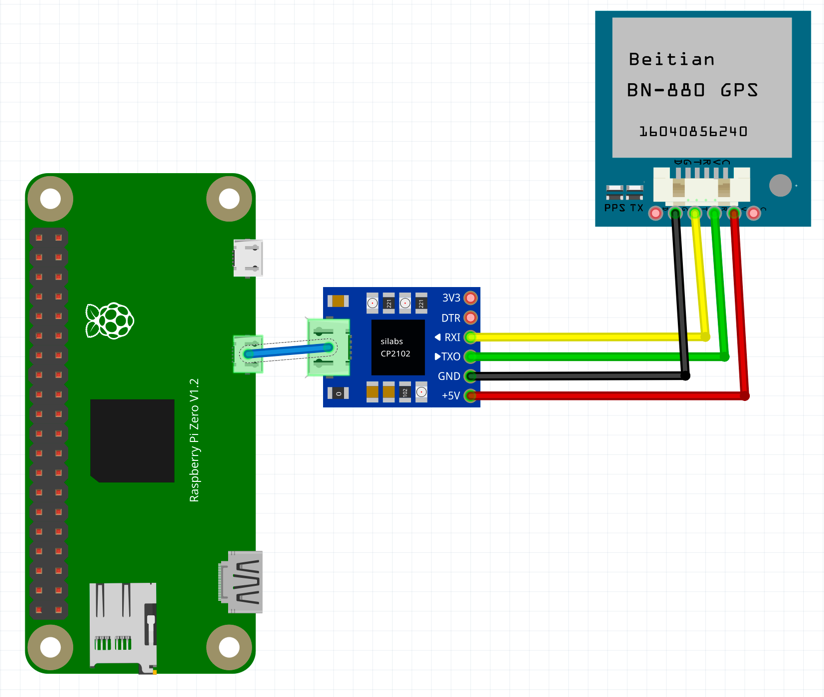
\includegraphics[width=0.7\textwidth]{Imagenes/Bitmap/conexion_gps}
        \caption{Diagrama de conexión del módulo GNSS BN-880 mediante el adaptador CP2102 }
        \label{fig:conexion_gps}
    \end{figure}
    \item \textbf{Cargador MCP73871:} es el encargado de gestionar la alimentación del sistema y la recarga de la batería.

    Este módulo permite cargar una batería de ion de litio y, simultáneamente, alimentar el sistema, conmutando automáticamente entre la entrada de alimentación externa y la batería según su disponibilidad.


    \begin{itemize}
        \item \textbf{Entrada de carga:} al conector USB-C hembra del módulo se conecta una entrada de alimentación externa.

        En este caso, se utilizan tres paneles solares de 2~V conectados en serie, cuyo cableado termina en un conector USB-C macho compatible con la entrada del cargador.

        \item \textbf{Conexión de la batería:} una batería de ion de litio de 3{,}7~V (tipo 18650) se conecta directamente a los terminales BAT+ y BAT- del módulo.

        Esta conexión permite tanto la carga de la batería como el suministro de energía al sistema cuando no hay entrada externa disponible.

        \item \textbf{Salida VBUS:} el terminal VBUS proporciona la tensión de salida activa en cada momento (procedente de la entrada USB-C o de la batería).

        Esta salida no está regulada y puede variar entre 3{,}7~V y 5{,}5~V, por lo que se conecta a un convertidor elevador (boost converter) que estabiliza la tensión a 5~V.

        La salida del boost se conecta al pin físico~2 (5~V) de la Raspberry Pi, y su masa al pin físico~39 (GND), proporcionando alimentación estable a todo el sistema.
    \end{itemize}
    \begin{figure}[H]
        \centering
        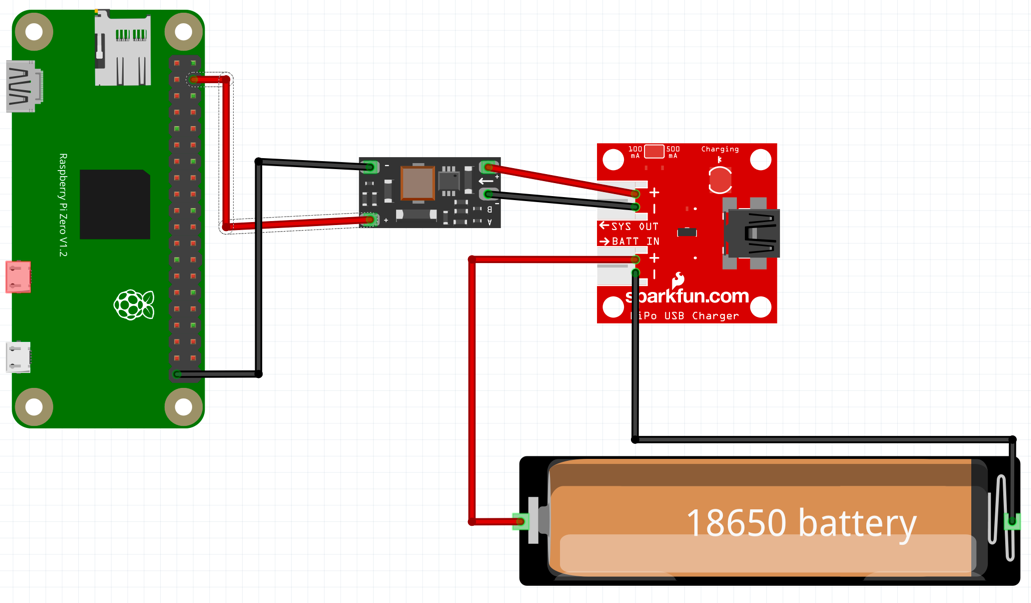
\includegraphics[width=0.7\textwidth]{Imagenes/Bitmap/conexion_cargador}
        \caption{Diagrama de conexión del cargador MCP73871 y booster}
        \label{fig:conexion_cargador}
    \end{figure}
    \item \textbf{Cámara CSI:} conectada directamente al puerto CSI (Camera Serial Interface) de la Raspberry Pi Zero 2 W mediante un cable plano.

    El puerto CSI es una interfaz específica para cámaras que permite transmitir vídeo sin utilizar pines GPIO.
    Además, proporciona tanto la alimentación como la señal de datos a través del propio conector.
\end{itemize}

\begin{table}[H]
    \centering
    \begin{tabular}{|l|l|l|l|}
        \hline
        \textbf{Módulo}     & \textbf{Función}     & \textbf{GPIO} & \textbf{Pin físico} \\ \hline
        BMP388              & SDA                  & GPIO 2        & 3                   \\ \cline{2-4}
        & SCL                  & GPIO 3        & 5                   \\ \cline{2-4}
        & VCC                  & -             & 1 (3.3 V)           \\ \cline{2-4}
        & GND                  & -             & 6                   \\ \hline
        BNO085              & SDA                  & GPIO 2        & 3                   \\ \cline{2-4}
        & SCL                  & GPIO 3        & 5                   \\ \cline{2-4}
        & VCC                  & -             & 1 (3.3 V)           \\ \cline{2-4}
        & GND                  & -             & 6                   \\ \hline
        LoRa E32-900T20D    & TX                   & GPIO 15       & 10                  \\ \cline{2-4}
        & RX                   & GPIO 14       & 8                   \\ \cline{2-4}
        & M0                   & GPIO 23       & 16                  \\ \cline{2-4}
        & M1                   & GPIO 24       & 18                  \\ \cline{2-4}
        & VCC                  & -             & 1 (5 V)             \\ \cline{2-4}
        & GND                  & -             & 6                   \\ \hline
        GNSS BN-880         & TX → RX del CP2102   & -             & -                   \\ \cline{2-4}
        & RX ← TX del CP2102   & -             & -                   \\ \cline{2-4}
        & VCC → VCC del CP2102 & -             & -                   \\ \cline{2-4}
        & GND → GND del CP2102 & -             & -                   \\ \hline
        Adaptador CP2102    & UART USB             & -             & Puerto USB (micro)  \\ \hline
        MCP73871 (cargador) & Entrada (USB-C)      & -             & -                   \\ \cline{2-4}
        & Salida a booster     & -             & -                   \\ \cline{2-4}
        & Boost out → Pi       & -             & 2 (5 V), 39 (GND)   \\ \hline
        Cámara CSI          & Datos + alimentación & -             & CSI                 \\ \hline
    \end{tabular}
    \caption{Resumen de conexiones de los periféricos a la Raspberry Pi Zero 2 W}
    \label{tab:resumen_conexiones}
\end{table}



A continuación se describe también el montaje de la estación de tierra, formada por un módulo LoRa conectado a una Raspberry Pi 4 a través de la interfaz UART:

\begin{itemize}
    \item TX del módulo → RX de la Pi: GPIO~15 (pin físico~10)
    \item RX del módulo ← TX de la Pi: GPIO~14 (pin físico~8)
    \item Pines M0 y M1: conectados respectivamente a los GPIO~23 (pin físico~16) y GPIO~24 (pin físico~18) de la Raspberry Pi, lo que permite gestionar el modo de operación del módulo desde software.
    \item Alimentación: 5~V (pin físico~2)
    \item GND: pin físico~6
    \item Conexión de antena: la antena externa se conecta al conector SMA hembra del módulo LoRa, permitiendo la comunicación en la banda de 868–915~MHz.

\end{itemize}

\begin{figure}[H]
    \centering
    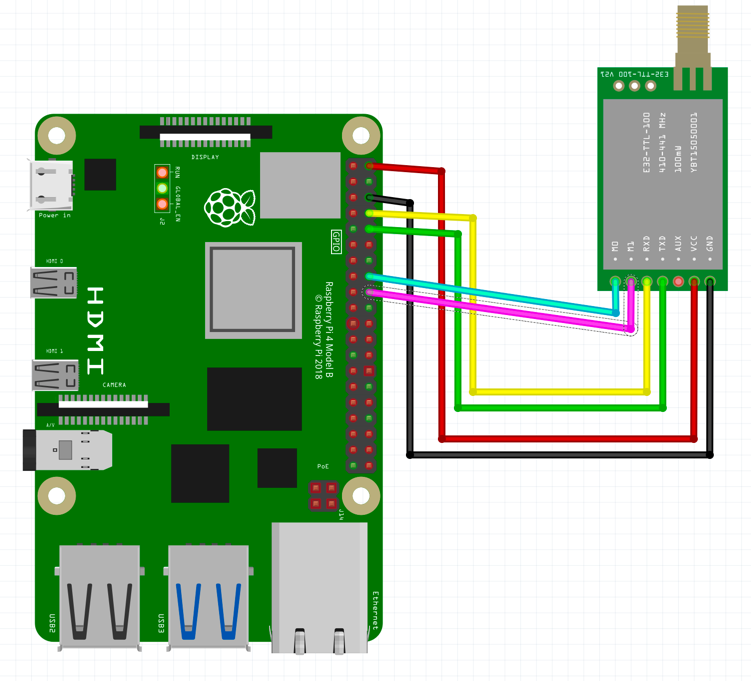
\includegraphics[width=0.7\textwidth]{Imagenes/Bitmap/conexion_ground}
    \caption{Diagrama de conexión de la estación de tierra con Raspberry Pi 4 y módulo LoRa}
    \label{fig:conexion_ground}
\end{figure}

\begin{table}[H]
    \centering
    \renewcommand{\arraystretch}{1.2}
    \begin{tabular}{|l|l|l|l|}
        \hline
        \textbf{Elemento} & \textbf{Función} & \textbf{GPIO} & \textbf{Pin físico} \\ \hline
        LoRa E32-900T20D  & TX → RX de la Pi & GPIO 15       & 10                  \\ \cline{2-4}
        & RX ← TX de la Pi & GPIO 14       & 8                   \\ \cline{2-4}
        & M0               & GPIO 23       & 16                  \\ \cline{2-4}
        & M1               & GPIO 24       & 18                  \\ \cline{2-4}
        & VCC              & --            & 2 (5 V)             \\ \cline{2-4}
        & GND              & --            & 6                   \\ \hline
    \end{tabular}
    \caption{Conexiones del módulo LoRa a la Raspberry Pi 4 en la estación de tierra}
    \label{tab:conexiones_ground_pi4}
\end{table}


Tras verificar el correcto funcionamiento de todas las conexiones en la protoboard, se procedió a su traslado a una placa PCB,
diseñada específicamente teniendo en cuenta las dimensiones y restricciones del CanSat.

\begin{figure}[H]
    \centering
    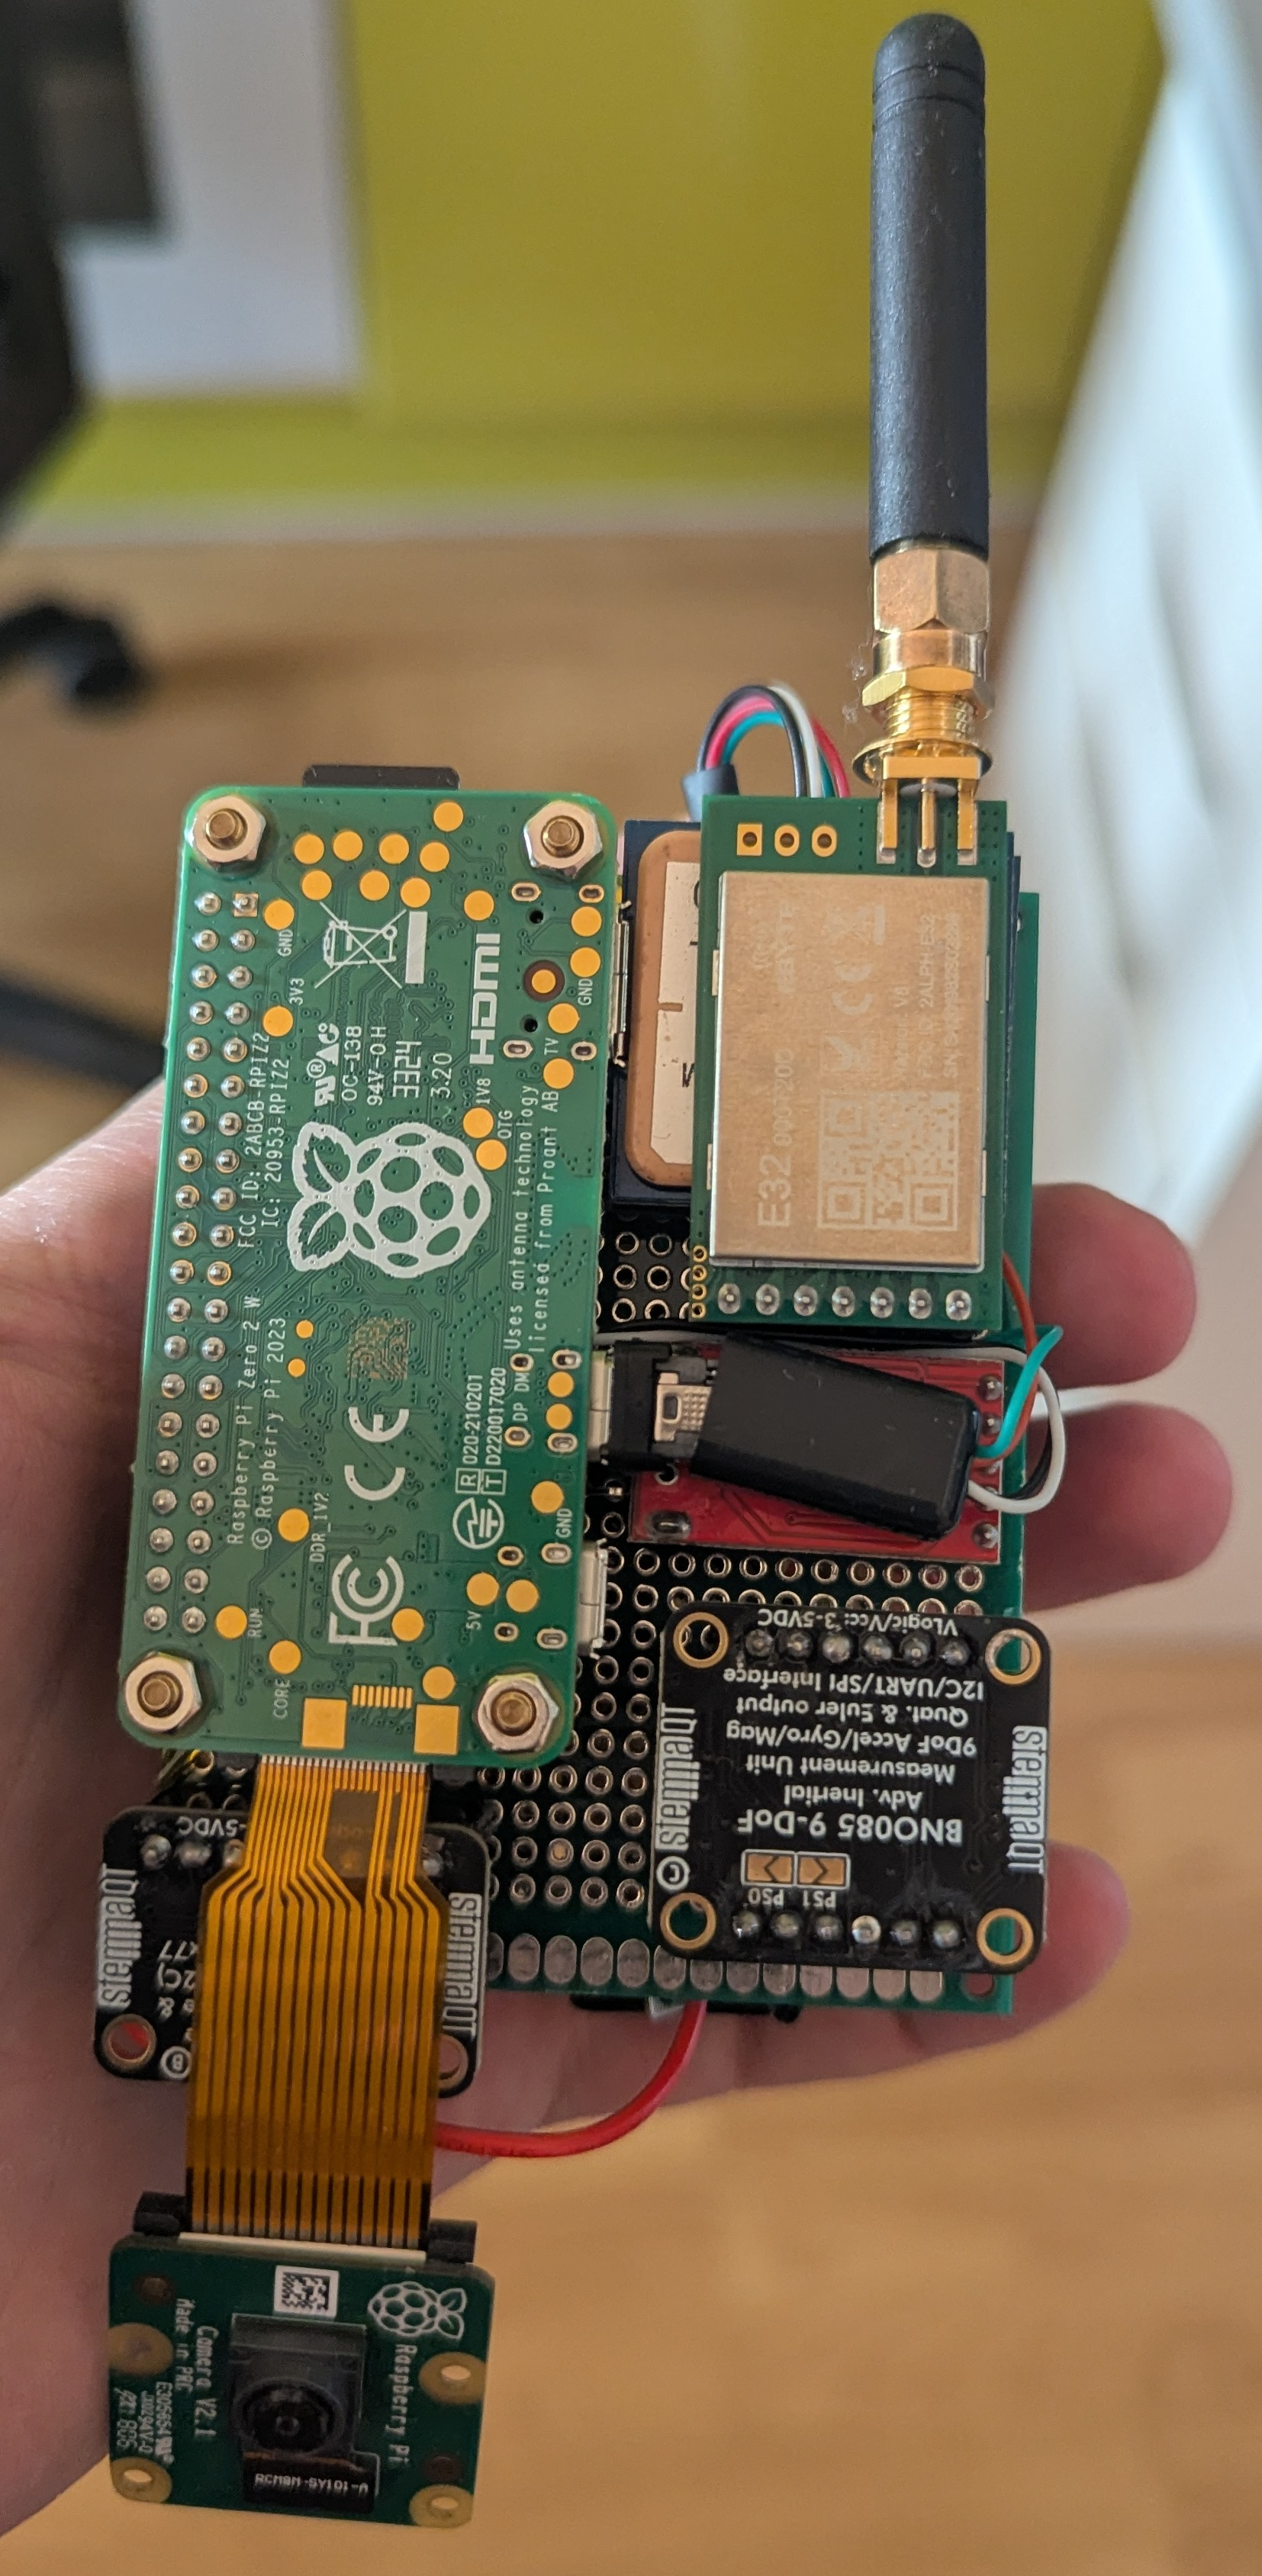
\includegraphics[width=0.3\textwidth]{Imagenes/Bitmap/pcb_montaje_frontal}
    \caption{Montaje final del sistema en la PCB (vista frontal)}
    \label{fig:pcb_montaje_frontal}
\end{figure}

\begin{figure}[H]
    \centering
    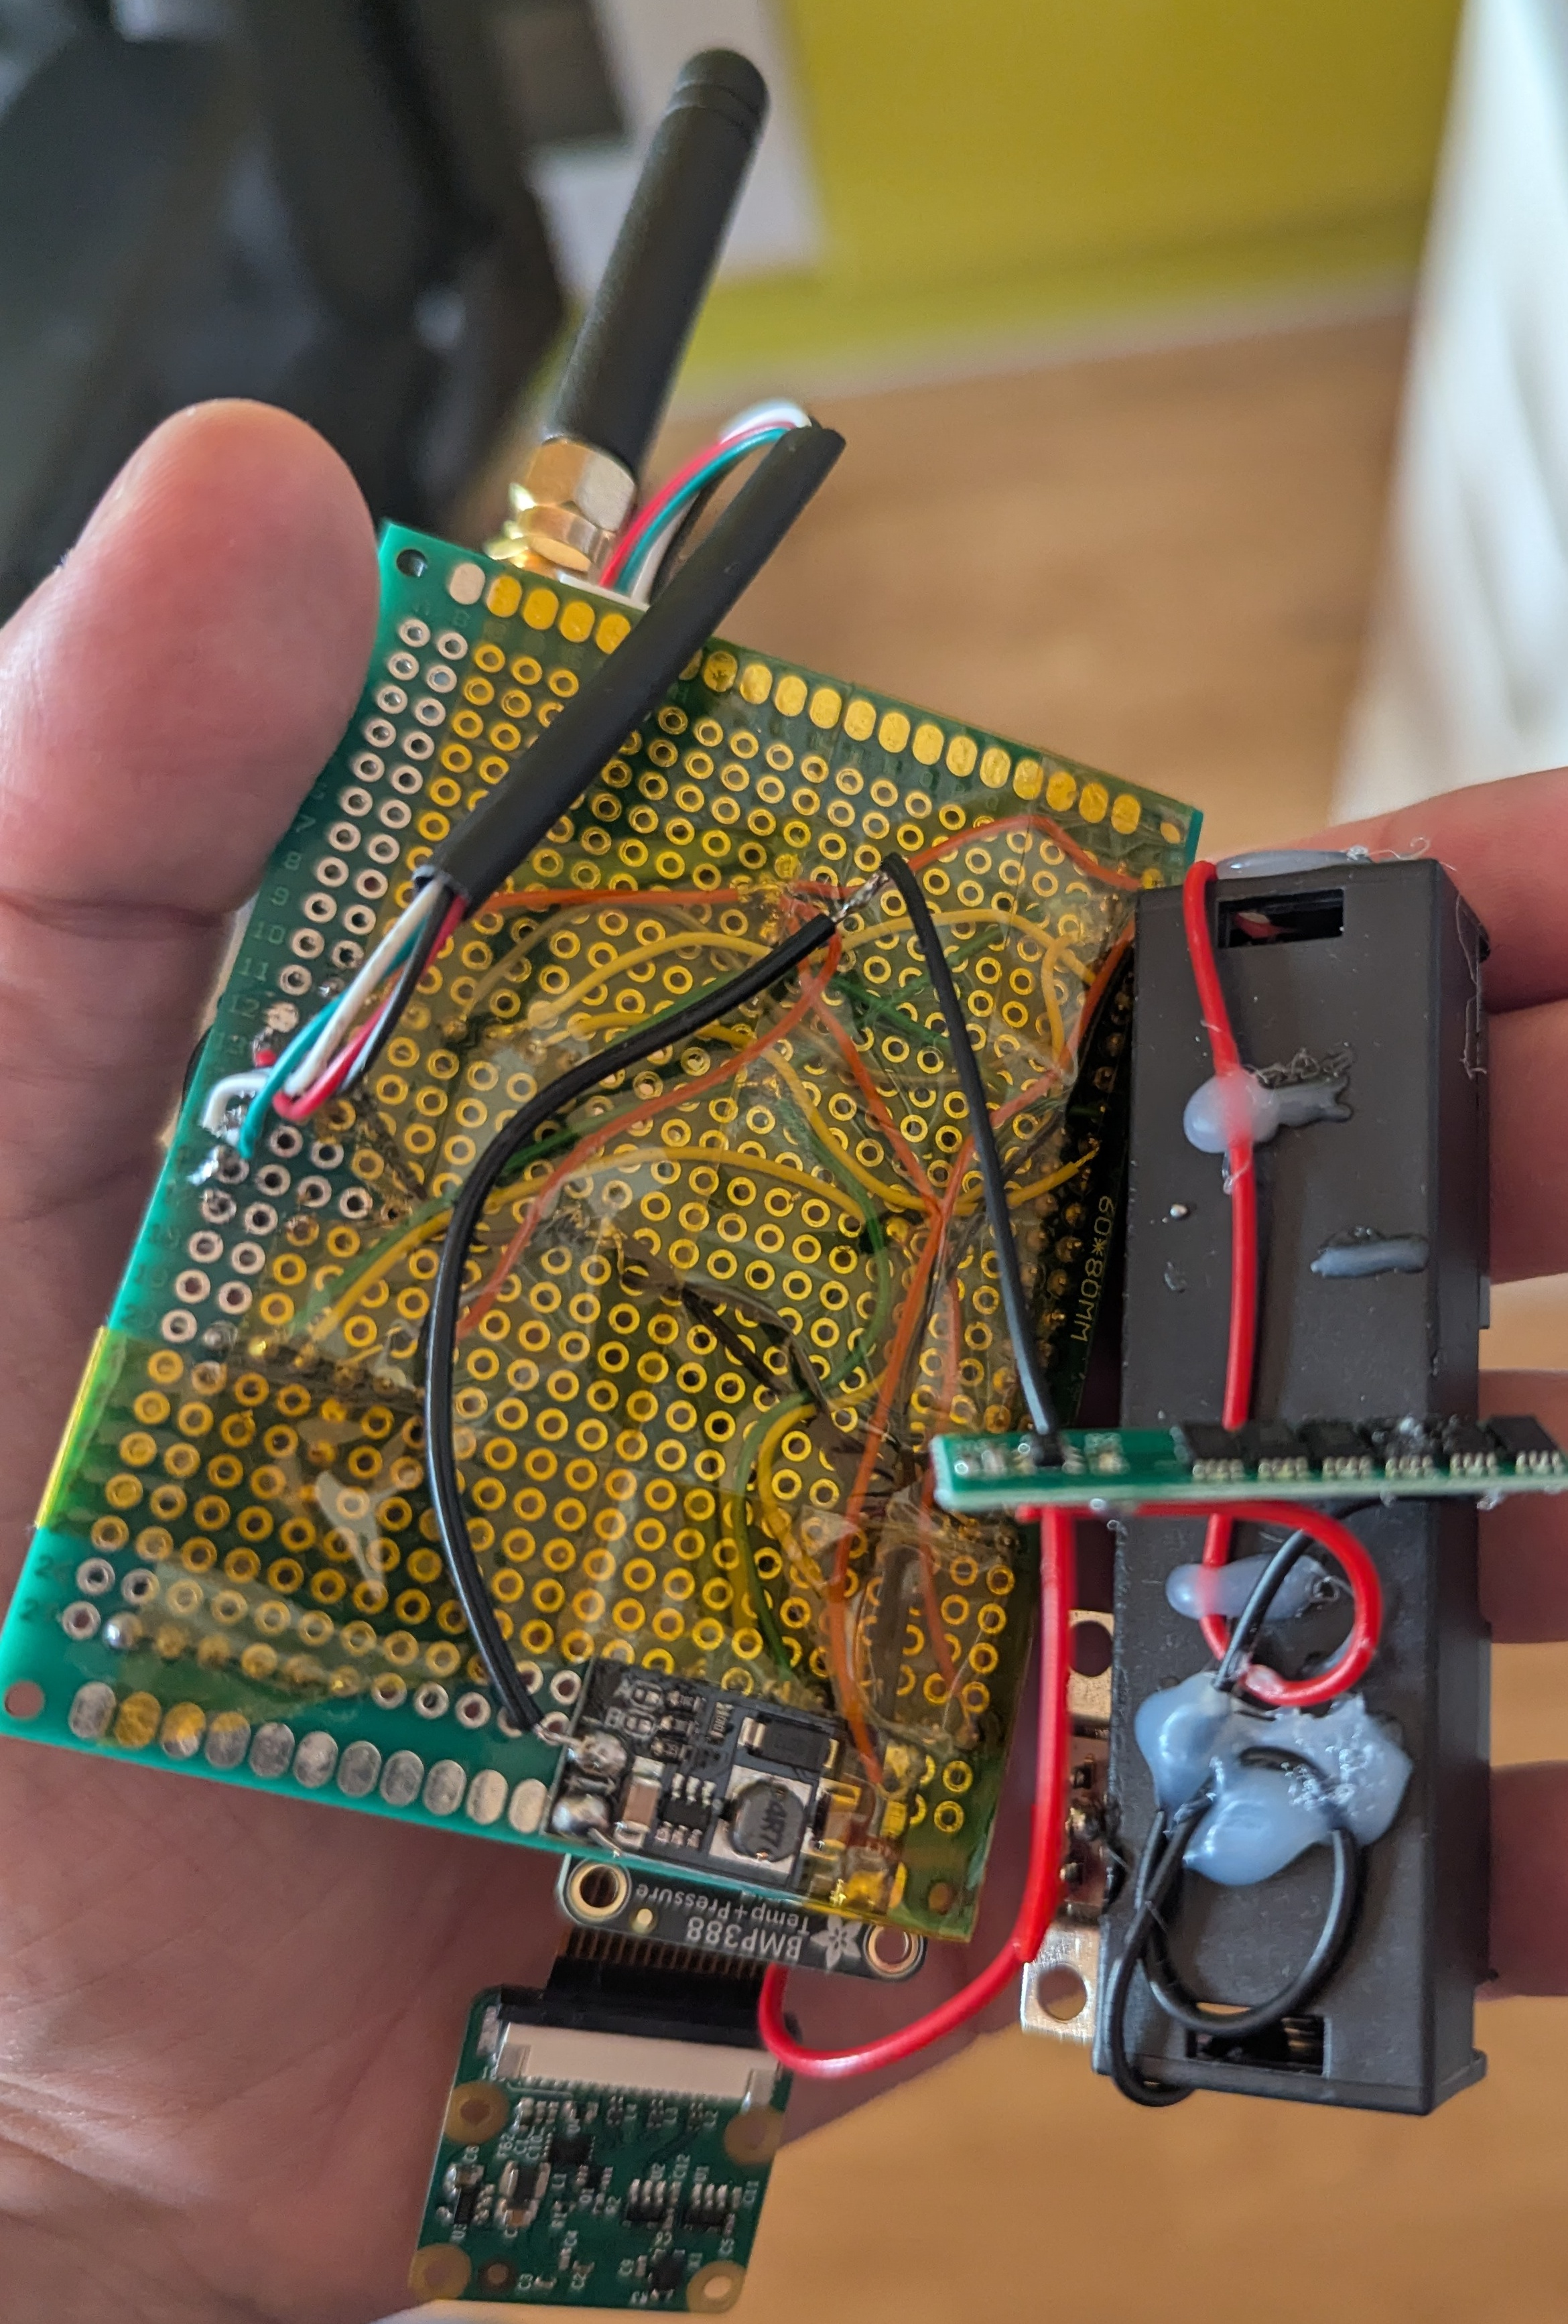
\includegraphics[width=0.5\textwidth]{Imagenes/Bitmap/pcb_montaje_trasero}
    \caption{Montaje final del sistema en la PCB (vista superior)}
    \label{fig:montaje_trasero}
\end{figure}


\section{Código embebido en la Raspberry Pi}

El código embebido desarrollado para la Raspberry Pi Zero 2~W está implementado en Python y se encarga de gestionar de forma concurrente la captura de vídeo, la adquisición de datos de sensores, el envío de eventos de telemetría por LoRa, y la publicación online a través de RabbitMQ.

El flujo de inicialización del sistema embebido sigue los siguientes pasos:

\begin{itemize}
    \item Esperar una conexión a internet durante 30 segundos para saber si debe enviar los datos mediante LoRa o publicarlos directamente en la cola de RabbitMQ.
    \item Crear una carpeta local donde se almacenarán los datos y vídeos generados, con nombre basado en la fecha y hora de arranque.
    \item Iniciar los módulos de captura de vídeo y envío de telemetría en hilos independientes.
\end{itemize}

\subsection{Captura de vídeo en tiempo real}

La clase \texttt{Camera} gestiona la captura de vídeo a través de la interfaz CSI usando la librería Picamera2.

El vídeo se guarda localmente y, si hay internet disponible, también se retransmite en directo mediante ffmpeg a un servidor RTMP externo.

El flujo de vídeo se configura con una resolución de 640x480 a 15~FPS, y se codifica en tiempo real con h264\_v4l2m2m para su emisión.

\subsection{Adquisición y envío de telemetría}

La clase \texttt{TelemetrySender} recopila información de múltiples sensores conectados a la Raspberry Pi:

\begin{itemize}
    \item \textbf{BMP388:} mide presión y temperatura atmosférica.
    Se accede a través de la librería adafruit\_bmp3xx.
    \item \textbf{BNO085:} proporciona la orientación del dispositivo (pitch, roll, yaw) a partir de cuaterniones.
    Se utiliza la librería adafruit\_bno08x.
    \item \textbf{BN-880 GNSS:} ofrece la posición geográfica, altitud GPS, velocidad y número de satélites.
    La información se decodifica a través de las librerías pyserial y pynmea2.
\end{itemize}

Estos datos se agregan en un evento del tipo TM con la fecha en la que se genera, este evento realiza el siguiente flujo:

\begin{itemize}
    \item Se generan cada 200~ms, agregando los datos más recientes de los sensores.
    \item Se publican en una cola RabbitMQ si hay conexión a internet.
    \item Se envían por LoRa mediante la clase \texttt{LoraSender} si no hay conexión a internet (máximo un evento cada 2 segundos).
    \item Se almacenan localmente en un fichero .jsonl.
\end{itemize}

\subsection{Envío por LoRa}

La clase \texttt{LoraSender} se encarga del envío de eventos en modo texto (CSV) a través del módulo LoRa.
Este envío se realiza en un hilo dedicado para no bloquear la adquisición de datos.

Después de envíar un evento sistema espera una confirmación OK durante un máximo de 2 segundos para considerar el envío exitoso y envíar el siguiente,
si no ese evento se descarta y se procede a envíar el siguiente, para ello se hace uso de una cola local.

\subsection{Conexión con RabbitMQ}

La clase \texttt{RabbitmqConnectionManager} crea y mantiene la conexión con el servidor RabbitMQ.

Publica los eventos codificados en JSON en el exchange tracking\_device\_events de tipo fanout.
Si la conexión se pierde, intenta restablecerla automáticamente.

\subsection{Formato de los eventos}

Cada evento tiene los siguientes campos principales:

\begin{itemize}
    \item \textbf{type:} tipo de evento (actualmente sólo TM para telemetría).
    \item \textbf{datetime:} fecha de la generación del evento formato ISO.
    \item \textbf{payload:} contiene todos los datos de sensores disponibles en ese instante.
\end{itemize}

Los eventos se serializan en formato JSON o CSV, en función del canal de transmisión utilizado (RabbitMQ o LoRa, respectivamente)


\section{Software de la estación de tierra}

El software de la estación de tierra está desarrollado en python y se encarga de realizar las siguientes acciones:

\begin{itemize}
    \item Intenta detectar si hay conexión a internet durante 30 segundos.
    Si se detecta conexión, el código continúa, en caso contrario, finaliza con un mensaje de error.
    \item Establece la conexión con el broker de RabbitMQ utilizando la clase \texttt{RabbitmqConnectionManager}.
    \item Espera hasta 30 segundos a que el puerto serie /dev/serial0 esté disponible y sea accesible.

    Una vez disponible, abre el puerto a una velocidad de 9600 baudios, este es el puerto en el que recibe los mensajes del módulo LoRa.
    \item Lee continuamente desde el puerto serie, acumulando los datos en un búfer hasta que detecta el delimitador \$, que indica el final de un mensaje.
    \item Intenta parsear el mensaje como un evento válido en formato CSV, usando la clase \texttt{Event}.

    Si el parseo se produce sin errores, convierte el evento a JSON y lo publica en RabbitMQ y responde por LoRa con un OK para confirmar la recepción.
    \item En caso de que el mensaje recibido está mal formado, lo descarta y registra el error sin interrumpir la ejecución.
    \item El sistema se puede detener mediante una interrupción por teclado (ctrl+C). Al cerrarse, libera el puerto serie y cierra la conexión con RabbitMQ de forma segura.
\end{itemize}


\section{Backend con Spring Boot}

El backend del sistema está desarrollado en Java utilizando el framework Spring Boot, es el encargado de recibir los eventos mediante RabbitMq, guardarlos en PostgreSQL y reenviarlos mediante WebSockets.

\subsection{Recepción de eventos}

Los eventos generados por el CanSat son enviados a RabbitMQ utilizando un exchange de tipo fanout llamado tracking\_device\_events.
El backend está suscrito a este exchange a través de una queue denominada tracking\_device\_events.dashboard\_backend, tal y como se configura en la clase \texttt{RabbitmqConfiguration}:

Cada vez que se recibe un mensaje en esta cola, el componente \texttt{TrackingDeviceEventsConsumer} se encarga de:
\begin{enumerate}
    \item Deserializar el evento desde JSON a un objeto \texttt{Event}.
    \item Guardar el evento en la base de datos a través del repositorio \texttt{EventJPA}.
    \item Publicar el evento a través de WebSocket mediante la clase \texttt{TrackingDeviceEventsProducer}.
\end{enumerate}

\subsection{Persistencia de eventos}

Los eventos se almacenan en una base de datos relacional mediante Spring Data JPA. Cada evento se representa con la clase \texttt{Event}, la cual contiene:
\begin{itemize}
    \item Un identificador único (id).
    \item El tipo de evento (type).
    \item La fecha y hora del evento (datetime).
    \item Un payload genérico como mapa clave-valor (Map<String, String>), almacenado como JSON en la base de datos.
\end{itemize}

\subsection{Acceso a eventos}

Se proporciona un endpoint REST para consultar eventos entre dos fechas:
\begin{itemize}
    \item \texttt{/events/range}: devuelve una lista de eventos como JSON.
    \item \texttt{/events/range/download}: permite descargar los eventos en formato JSONL.
\end{itemize}

\subsection{Distribución en tiempo real}

El backend incluye soporte para WebSocket, los eventos almacenados se reenvían al canal \texttt{/topic/events} a través de la clase \texttt{TrackingDeviceEventsProducer}.


\section{Frontend con Flutter para visualización en tiempo real}

El frontend ha sido desarrollado utilizando Flutter, permitiendo desplegar una aplicación web responsive capaz de visualizar los eventos emitidos por el CanSat.
La comunicación con el backend se realiza a través de WebSocket, suscribiéndose al canal /topic/events.

La interfaz ha sido diseñada con el objetivo de ser lo más genérica posible, facilitando la visualización de métricas y gráficas sin atarse a una configuración de sensores específica o a un diseño de CanSat concreto.
Esto permite adaptar fácilmente la plataforma a otros proyectos con diferentes sensores o estructuras.

\subsection{Arquitectura general}

La aplicación se estructura en torno a un patrón BLoC (Business Logic Component), donde el estado del último evento recibido se propaga de forma reactiva a los distintos widgets encargados de representar la telemetría.

El componente principal TrackingDeviceEventBloc inicializa el cliente de WebSocket, gestiona la conexión y parsea los mensajes entrantes desde el backend,
convirtiéndolos en instancias de la clase \texttt{Event}.
Esta clase encapsula tanto la fecha como el tipo de evento y su carga útil (payload).

\subsection{Visualización modular}

La interfaz gráfica se divide en varios componentes:

\begin{itemize}
    \item \textbf{Metrics:} muestra el último valor de todos los parámetros y una lista de todos los eventos de telemetría recibidos.

    También permite la descarga de eventos históricos en formato .jsonl especificando un rango de fechas.
    \begin{figure}[H]
        \centering
        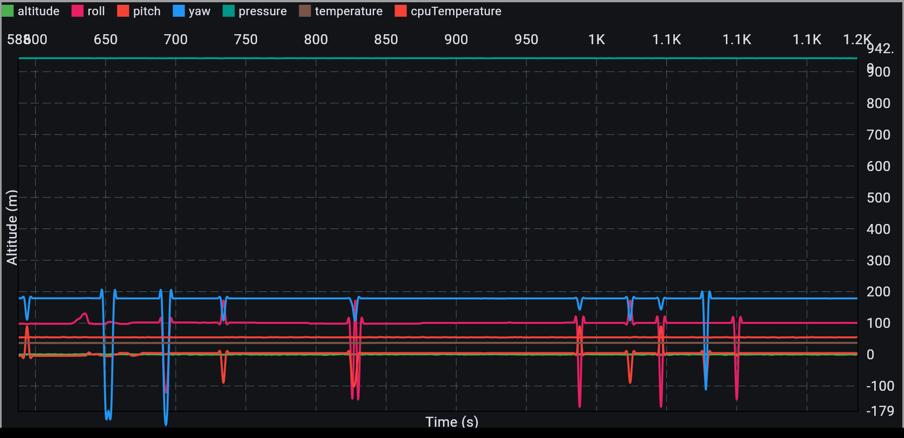
\includegraphics[width=0.8\textwidth]{Imagenes/Bitmap/metrics}
        \caption{Ejemplo del Componente Metrics}
        \label{fig:metrics}
    \end{figure}
    \item \textbf{Attitude:} renderiza un modelo tridimensional que rota en tiempo real según los valores de yaw, pitch y roll incluidos en cada evento, de esta manera es posible ver la orientación actual del CanSat.
    \begin{figure}[H]
        \centering
        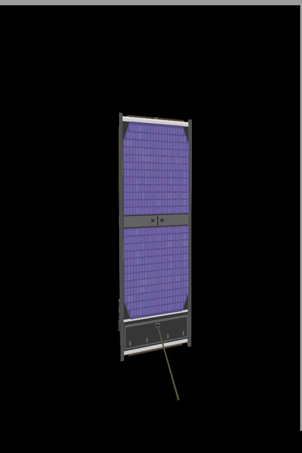
\includegraphics[width=0.4\textwidth]{Imagenes/Bitmap/attitude}
        \caption{Ejemplo del Componente Attitude}
        \label{fig:attitude}
    \end{figure}
    \item \textbf{TelemetryChart:} representa todos los valores de los parámetros recibidos como gráficas temporales utilizando, permitiendo observar la evolución de múltiples variables simultáneamente.
    \begin{figure}[H]
        \centering
        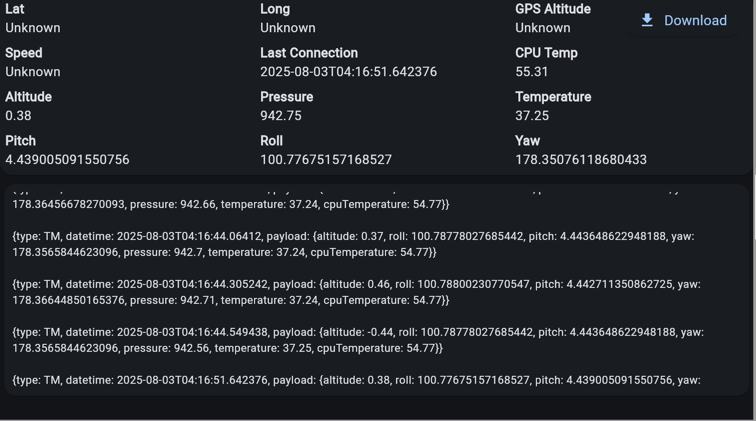
\includegraphics[width=0.8\textwidth]{Imagenes/Bitmap/telemetry_chart}
        \caption{Ejemplo del Componente TelemetryChart}
        \label{fig:telemetry_chart}
    \end{figure}
    \item \textbf{Map:} muestra un mapa con la última ubicación recibida del CanSat.
    \begin{figure}[H]
        \centering
        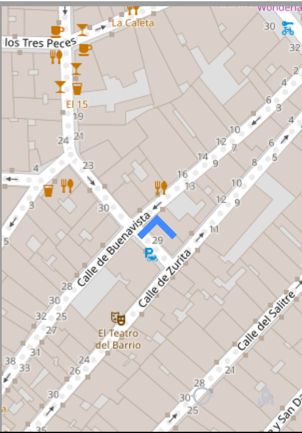
\includegraphics[width=0.4\textwidth]{Imagenes/Bitmap/map}
        \caption{Ejemplo del Componente Map}
        \label{fig:map}
    \end{figure}
    \item \textbf{Camera:} muestra la retransmisión de vídeo en directo.
\end{itemize}
\begin{figure}[H]
    \centering
    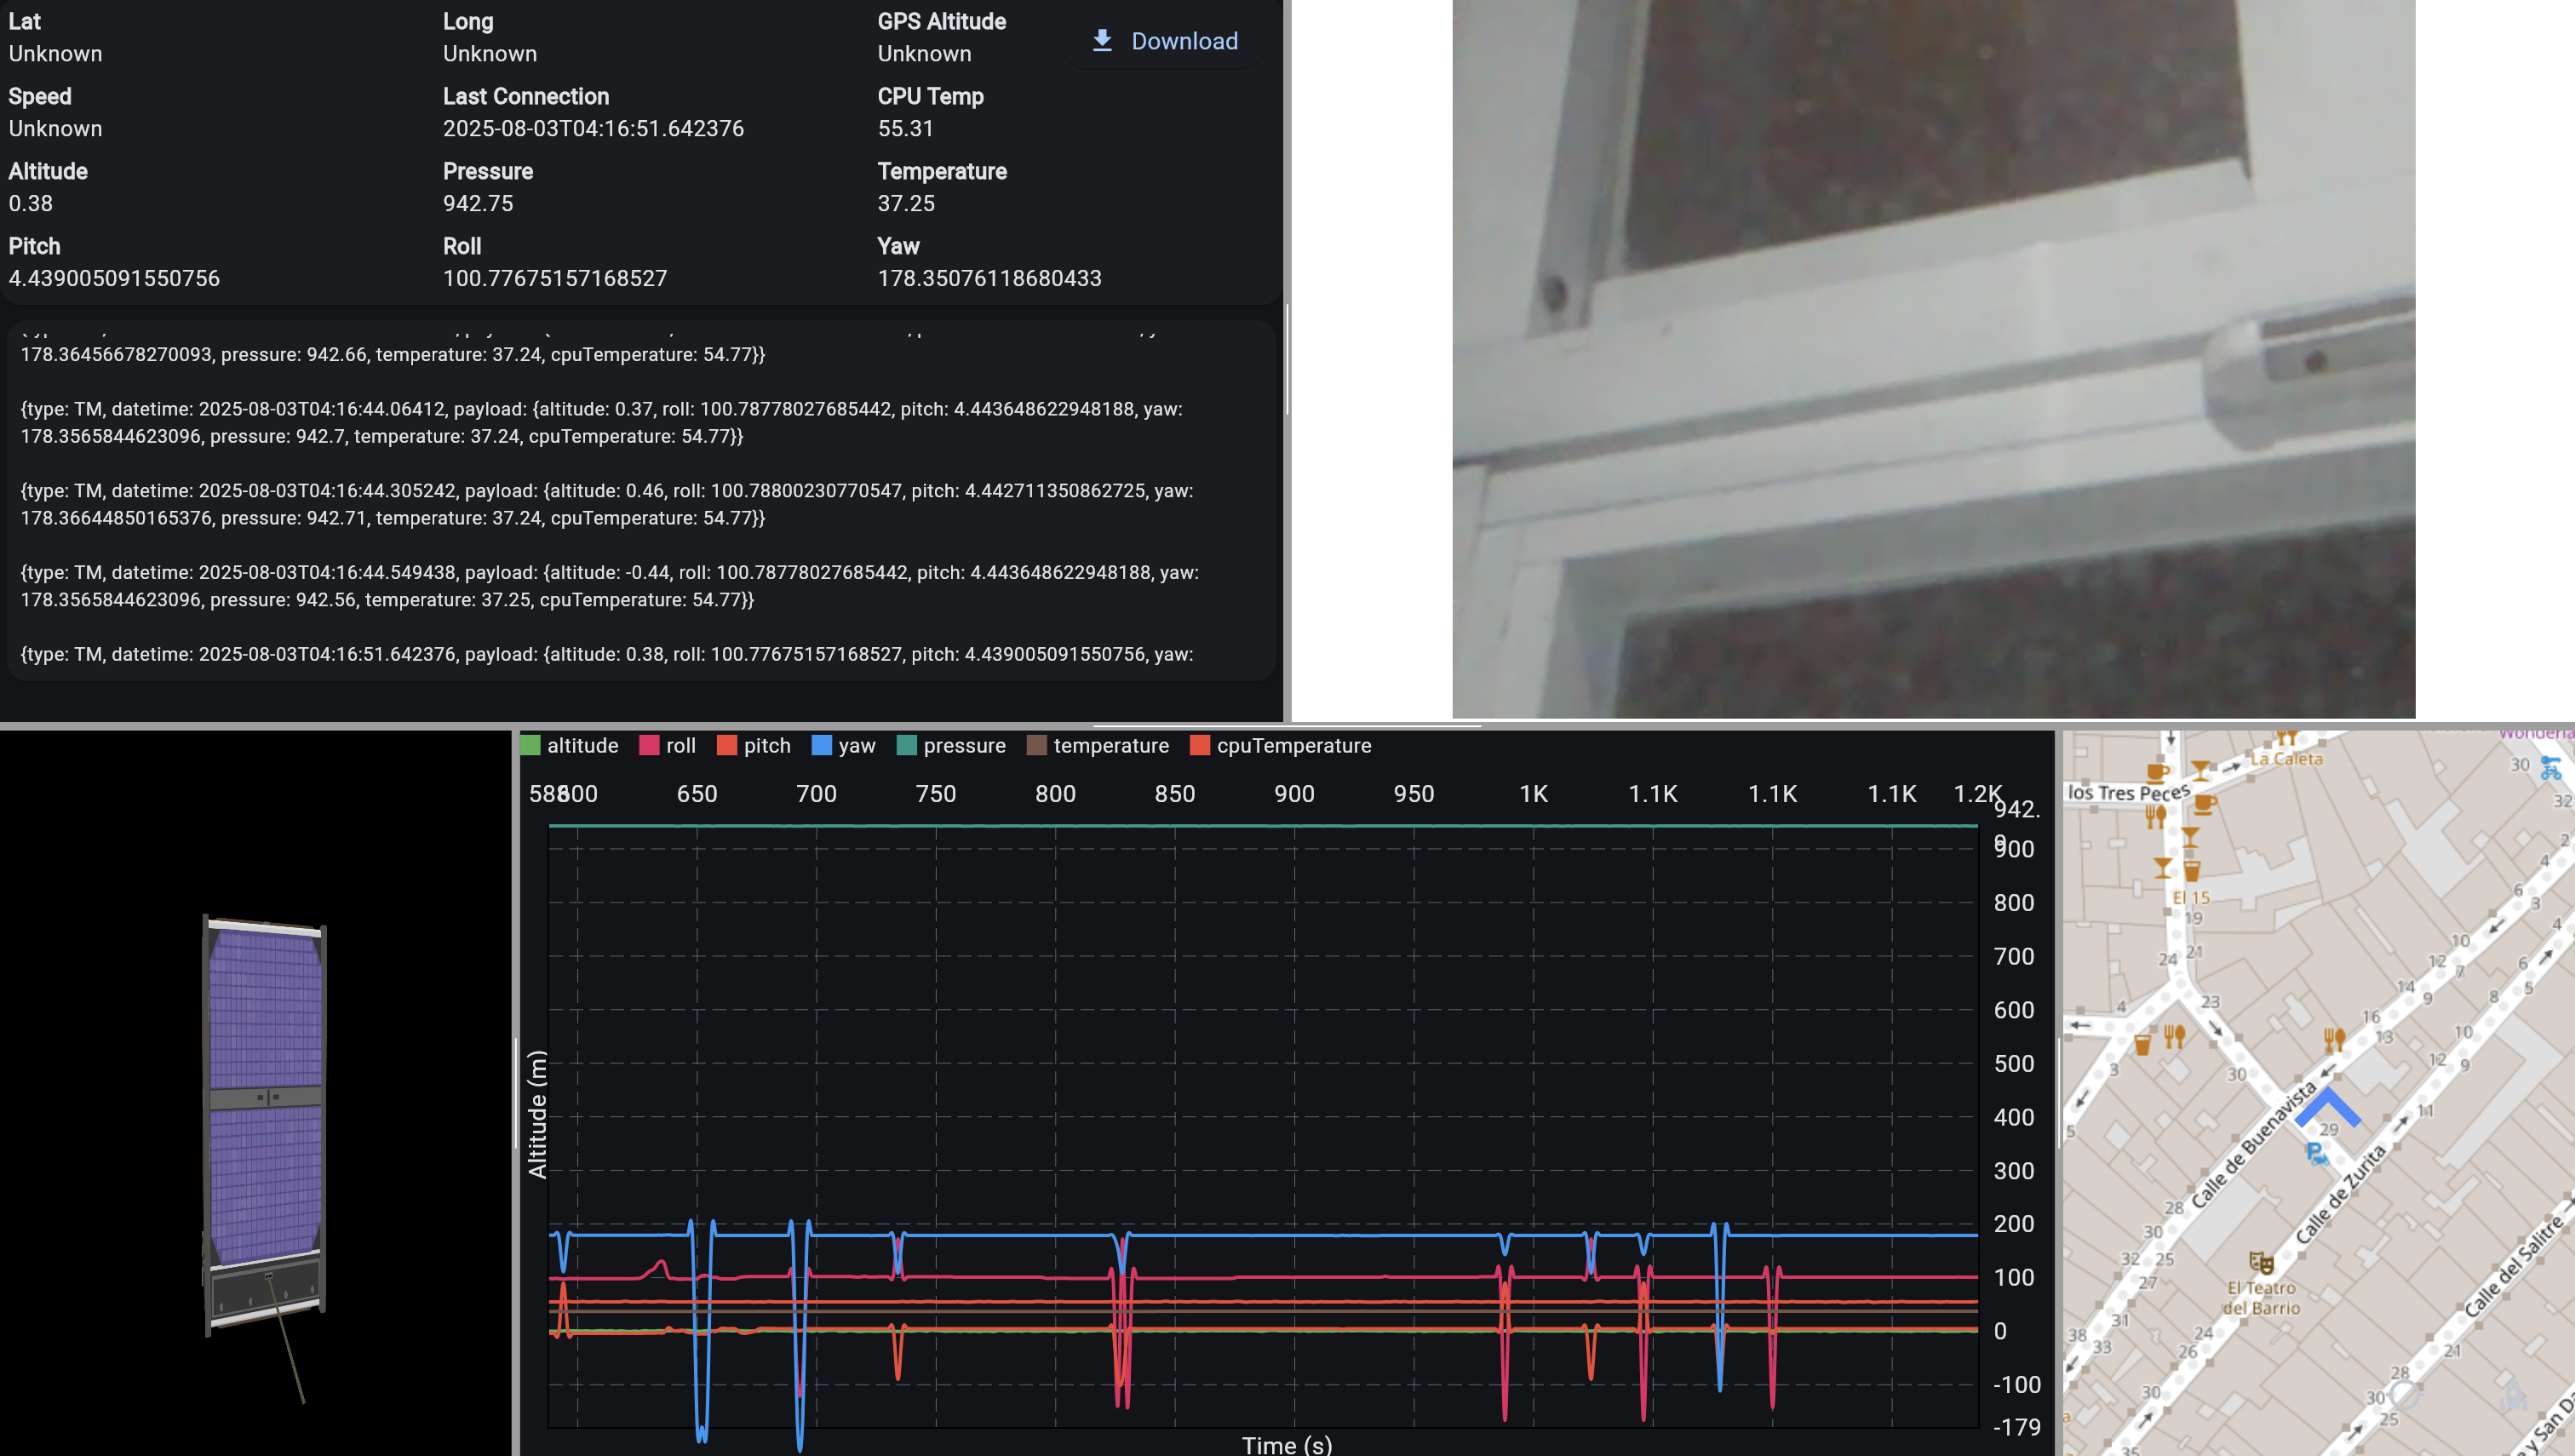
\includegraphics[width=1\textwidth]{Imagenes/Bitmap/initerfaz_general}
    \caption{Interfaz en modo escritorio}
    \label{fig:interfaz_general}
\end{figure}

\subsection{Adaptabilidad}

El diseño de la interfaz se adapta automáticamente a la resolución de pantalla.
En escritorio el espacio se divide en secciones horizontales y verticales que pueden ser redimensionadas de manera independiente, mientras que en móviles los elementos se muestran uno debajo de otro.


\section{Pruebas de integración y validación}


%\include{Capitulos/Capitulo4}
%\include{Capitulos/Capitulo5}
\chapter{Conclusiones y Trabajo Futuro}
\label{cap:conclusiones}

El objetivo principal que se planteaba al inicio del trabajo de crear una plataforma de visualización de datos en tiempo real, reutilizable y desacoplada de hardware específico ha sido cumplido.
Esto se ha conseguido gracias al análisis de otras soluciones existentes y al diseño de una arquitectura centrada, desde sus primeras fases, en la independencia del hardware y en su integración sencilla en otros proyectos.

La arquitectura modular del sistema facilita su mantenimiento y evolución.
Cada componente (captura de datos, transmisión, backend, frontend) puede modificarse de manera independiente sin afectar al resto del sistema, lo que permite su reutilización parcial.

La construcción de un CanSat ha servido como caso ejemplo para validar la plataforma, confirmando que no existen dependencias entre el sistema de visualización y el hardware.
Este ejemplo demuestra que la solución puede adaptarse fácilmente a configuraciones de sensores, protocolos o arquitecturas de CanSat distintas.

Además, el desarrollo del flujo completo, desde la adquisición de datos hasta su visualización en tiempo real, ha permitido identificar puntos críticos,
permitiendo optimizar los tiempos de transmisión y garantizar la sincronización de eventos en entornos reales.

En conjunto, el trabajo ha generado una plataforma flexible, útil no solo como solución cerrada,
sino como punto de partida para futuros desarrollos en proyectos con necesidades similares de visualización de datos.

A pesar de haber alcanzado los objetivos inicialmente propuestos, se han identificado
varias líneas de mejora en las que trabajar en el futuro:

\begin{itemize}
    \item Aumentar el número de gráficas disponibles en la aplicación web, incorporando visualizaciones específicas para determinados parámetros.
    \item Implementar un sistema de envío de telecomandos al CanSat para manejar su configuración de manera remota, esto permitiría activar o desactivar sensores o modificar parámetros como el intervalo de envío de datos directamente en tiempo de ejecución.
    \item Implementar un sistema de autenticación en la aplicación web para proteger posibles datos sensibles.
    \item Añadir soporte para visualizar múltiples CanSat al mismo tiempo. Actualmente no se distingue el origen de los eventos, por lo que no es posible monitorizar varios dispositivos simultáneamente.
    \item El desarrollo del CanSat se ha centrado en la parte electrónica y de software, se podría crear una carcasa 3D y un paracaídas para poder usarlo en lanzamientos reales.
\end{itemize}










%%%%%%%%%%%%%%%%%%%%%%%%%%%%%%%%%%%%%%%%%%%%%%%%%%%%%%%%%%%%%%%%%%%%%%%%%%%
% Si el TFM se escribe en inglés, comentar las siguientes líneas 
% porque no es necesario incluir nuevamente las Conclusiones en inglés
\begin{otherlanguage}{english}
\chapter{Introduction}
\label{cap:introduction}

This Master's Thesis presents the design and implementation of a complete system for real-time data acquisition, transmission, and visualization inspired by the CanSat concept, whose basic structure is shown in Figure~\ref{fig:cansate}.

The project consists of the construction of a CanSat-type device with different sensors, a Global Navigation Satellite System (GNSS) module, a camera, and communication via Wi-Fi or radio, as well as an open-source web platform in charge of visualizing the collected data in real time.

The platform has been designed as a generic and reusable tool, making it easy to adapt to other similar projects.  
Throughout this document, the context of the work, the motivation, the objectives, the planning, and the overall structure of the thesis are described.

\begin{figure}
    \centering
    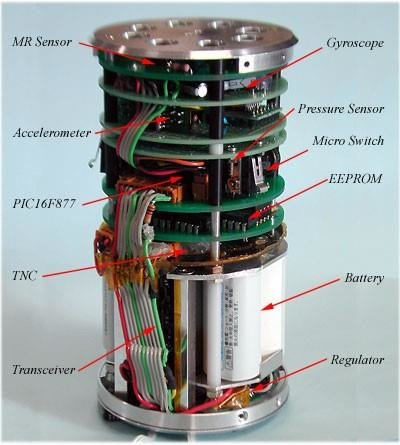
\includegraphics[width=0.5\textwidth]{Imagenes/Bitmap/cansat}
    \caption{Basic diagram of a CanSat. Source: \cite{researchgate_cansat2018}}
    \label{fig:cansate}
\end{figure}

\section{Context}
The CanSat project, whose name comes from the combination of the words \emph{can} and \emph{satellite}, was proposed by Professor Robert J. Twiggs in 1998~\cite{jaxa_cansat}.  
It began as an educational project simulating a nanosatellite with the size of a soda can and a weight of about 350 grams.  
Its objective is to help students of different levels understand all the phases involved in the development of a satellite, from defining the scientific mission to integrating the complete system, including the required sensors, the electronics for operation, the radio transmission to a ground station, the visualization of the data, the design of a 3D-printed enclosure capable of withstanding launch forces, and the design of a parachute.

CanSats are not put into orbit but launched by model rockets, high-altitude balloons, or drones. They are thus subjected to external forces such as acceleration, vibration, or possible impacts, which makes it necessary for them to have a resistant structure.  
The mission of a CanSat is to use its sensors to collect data during descent and transmit them to the ground station.

In recent years, the popularity of CanSats has increased, leading to the creation of national and international competitions promoted by space agencies such as the European Space Agency~\cite{esa_cansat2024}, with the aim of encouraging interest in the aerospace sector and STEM careers in general from an early age.

\section{Motivation}
These projects usually focus on the electronic aspects (data acquisition and transmission), while the visualization of the data often remains underdeveloped.  
In many cases, only basic solutions are implemented, such as console-based visualization or simple plots.  
Moreover, these solutions are often tied to a specific CanSat, which forces each new project to build its visualization solution from scratch.

This highlights the need for a common and reusable platform that allows the real-time visualization of data sent by the CanSat and received by the antenna in a professional and visually clear way, without depending on specific hardware.  
Such a platform would facilitate data analysis during testing and launches and could serve as a base for future project-specific implementations, helping students integrate advanced visualizations without needing to develop a complete platform themselves.

\section{Objectives}
The main objective of this project is to design and develop from scratch a CanSat-type satellite and to implement a reusable data visualization platform.  
The objectives were divided into two main parts: technology research and CanSat development.  
The steps followed in each part are described below.

\begin{itemize}
    \item \textbf{Research}
    \begin{itemize}
        \item Comparison of different microcontrollers and single-board computers to determine which best fit the project objectives.
        \item Study of available sensors on the market and their communication with the microcomputer.
        \item Analysis of different power supply options for the CanSat, including the possibility of using solar panels.
        \item Comparison of current data visualization tools.
    \end{itemize}
    \item \textbf{Development}, divided into two parts: CanSat hardware creation and the visualization platform.
    \begin{itemize}
        \item CanSat
        \begin{itemize}
            \item Construction of a CanSat that complies with the basic size (66 mm × 115 mm) and weight (300–350 g) requirements.
            \item Integration of a GPS receiver.
            \item Camera for real-time video transmission.
            \item Sensors for pressure, temperature, and altitude.
            \item Gyroscope for device orientation.
            \item Battery with solar charging capability.
            \item Data transmission via Wi-Fi when an internet connection is available.
            \item Data transmission via radio when no internet connection is available.
            \item Development of a ground radio receiver.
        \end{itemize}
        \item Visualization platform
        \begin{itemize}
            \item Real-time visualization of all telemetry data received.
            \item Display of the most recent value of each telemetry parameter.
            \item Real-time plots of the received values.
            \item Real-time visualization of transmitted images.
            \item Map with the exact location of the CanSat.
            \item 3D model showing the actual orientation of the CanSat.
            \item Telemetry data download for a selected date range.
        \end{itemize}
    \end{itemize}
\end{itemize}

\section{Work Plan}
The project followed a structured work plan to organize tasks and achieve the proposed objectives.  
This plan was divided into the following steps:

\begin{itemize}
    \item Review and comparison of Arduino and ESP32 microcontrollers and the Raspberry Pi Zero 2 single-board computer, based on their capabilities and compatibility with sensors and communication modules.
    \item Selection of sensors (GNSS, altimeter, and gyroscope), communication module, camera, and power system.
    \item Initial assembly of components on prototyping boards to simplify individual testing.
    \item Definition of the general system architecture, composed of three main components:
    \begin{itemize}
        \item Embedded code in the Raspberry Pi for sensor reading and data transmission.
        \item Ground radio receiver for data sent by the CanSat.
        \item Real-time visualization platform.
    \end{itemize}
    \item Implementation of embedded code on the Raspberry Pi using Python and the appropriate libraries for each sensor.
    \item Implementation of the real-time visualization platform based on events, using RabbitMQ as a message broker, a Java Spring Boot \emph{backend}, a Flutter \emph{frontend}, and a PostgreSQL database to store telemetry data.
    \item Soldering of the components onto a final PCB that complies with the CanSat size requirements.
    \item Integration testing of the complete system, including battery lifetime tests and radio communication range tests.
    \item Writing of the thesis, documenting all steps and results.
\end{itemize}

\section{Source Code and License}
All code developed for this project is available in a single public repository under the MIT license.  
It includes the backend, frontend, and the embedded scripts for both the CanSat and the ground station.  
The repository is hosted on GitHub:

\url{https://github.com/tronxi/real-time-tracking-system}

\section{Thesis Structure}
The thesis is organized into the following chapters:

\begin{itemize}
    \item \textbf{Chapter 1. Introduction:} presents the project context, personal and academic motivation, objectives, and work plan.
    \item \textbf{Chapter 2. Related Work:} reviews previous initiatives related to the CanSat concept, both educational and technical, and analyzes different solutions for data acquisition, transmission, and visualization.
    \item \textbf{Chapter 3. Theoretical Foundations:} defines the technical concepts required for system development, including hardware comparisons, communication technologies, sensors, video protocols, and real-time visualization architectures.
    \item \textbf{Chapter 4. System Design and Implementation:} describes the complete system architecture, the chosen components, the CanSat assembly, the embedded software, the backend, the frontend, and the performed tests.
    \item \textbf{Chapter 5. Conclusions and Future Work:} summarizes the main conclusions of the work, evaluates the results, and proposes possible improvements and future research directions.
\end{itemize}









\chapter{Conclusions and Future Work}
\label{cap:conclusions}

The main objective set at the beginning of this work, to create a real-time data 
visualization platform that is reusable and decoupled from specific hardware, has been 
achieved. This was accomplished through the analysis of existing solutions and the design 
of an architecture focused, from its earliest stages, on hardware independence and 
straightforward integration into other projects.

The modular architecture of the system facilitates its maintenance and evolution. Each 
component (data acquisition, transmission, backend, frontend) can be 
modified independently without affecting the rest of the system, which allows for partial 
reuse.

The construction of a CanSat has served as a case study to validate the platform, 
confirming that there are no dependencies between the visualization system and the 
hardware. This example demonstrates that the solution can be easily adapted to different 
sensor configurations, protocols, or CanSat architectures.

The development of the complete workflow, from data acquisition to real-time 
visualization, made it possible to identify critical points and optimize transmission 
times, ensuring event synchronization in real environments. As a result, the project has 
produced a flexible platform, useful not only as a standalone solution but also as a 
foundation for future developments in projects with similar data visualization needs.

During the development, several challenges also had to be addressed. One of the most 
significant was the Raspberry Pi Zero~2~W, which showed limitations in reliably managing 
real-time video streaming. To make it work, it was necessary to reduce the resolution to 
640×480 pixels and the frame rate to 15~fps, as well as to use ffmpeg with 
hardware-accelerated H.264 encoding. These optimizations allowed the video stream to be 
transmitted continuously to the RTMP server, ensuring uninterrupted visualization on the 
web application.

Another issue was related to the connection of the BN-880 GNSS receiver. This Raspberry 
model provides only one UART port accessible through the GPIOs, which in this case was 
already used by the LoRa module. To add the GNSS, it was necessary to use a USB–UART 
adapter based on the CP2102 chip. Due to the limited available space, the adapter had to 
be physically modified by removing the original connector and soldering a more compact 
micro-USB. This adaptation made it possible to integrate the GNSS into the system without 
exceeding the maximum dimensions of the CanSat.

Finally, several lines of improvement have been identified for future work:

\begin{itemize}
    \item Expand the number of charts in the web application, adding visualizations for specific parameters.
    \item Add a telecommand system to manage the CanSat remotely. This would allow enabling or disabling sensors or changing parameters such as the data transmission interval at runtime.
    \item Introduce an authentication system in the web application to protect sensitive data.
    \item Support simultaneous visualization of multiple CanSats. At present, the origin of events is not distinguished, which prevents monitoring several devices at the same time.
    \item Extend the development of the CanSat beyond electronics and software with a 3D-printed enclosure and a parachute to enable real launch operations.
\end{itemize}




\end{otherlanguage}
%%%%%%%%%%%%%%%%%%%%%%%%%%%%%%%%%%%%%%%%%%%%%%%%%%%%%%%%%%%%%%%%%%%%%%%%%%%

%
% Bibliografía
%
% Si el TFM se escribe en inglés, editar TeXiS/TeXiS_bib para cambiar el
% estilo de las referencias
%---------------------------------------------------------------------
%
%                      configBibliografia.tex
%
%---------------------------------------------------------------------
%
% bibliografia.tex
% Copyright 2009 Marco Antonio Gomez-Martin, Pedro Pablo Gomez-Martin
%
% This file belongs to the TeXiS manual, a LaTeX template for writting
% Thesis and other documents. The complete last TeXiS package can
% be obtained from http://gaia.fdi.ucm.es/projects/texis/
%
% Although the TeXiS template itself is distributed under the 
% conditions of the LaTeX Project Public License
% (http://www.latex-project.org/lppl.txt), the manual content
% uses the CC-BY-SA license that stays that you are free:
%
%    - to share & to copy, distribute and transmit the work
%    - to remix and to adapt the work
%
% under the following conditions:
%
%    - Attribution: you must attribute the work in the manner
%      specified by the author or licensor (but not in any way that
%      suggests that they endorse you or your use of the work).
%    - Share Alike: if you alter, transform, or build upon this
%      work, you may distribute the resulting work only under the
%      same, similar or a compatible license.
%
% The complete license is available in
% http://creativecommons.org/licenses/by-sa/3.0/legalcode
%
%---------------------------------------------------------------------
%
% Fichero  que  configura  los  parámetros  de  la  generación  de  la
% bibliografía.  Existen dos  parámetros configurables:  los ficheros
% .bib que se utilizan y la frase célebre que aparece justo antes de la
% primera referencia.
%
%---------------------------------------------------------------------


%%%%%%%%%%%%%%%%%%%%%%%%%%%%%%%%%%%%%%%%%%%%%%%%%%%%%%%%%%%%%%%%%%%%%%
% Definición de los ficheros .bib utilizados:
% \setBibFiles{<lista ficheros sin extension, separados por comas>}
% Nota:
% Es IMPORTANTE que los ficheros estén en la misma línea que
% el comando \setBibFiles. Si se desea utilizar varias líneas,
% terminarlas con una apertura de comentario.
%%%%%%%%%%%%%%%%%%%%%%%%%%%%%%%%%%%%%%%%%%%%%%%%%%%%%%%%%%%%%%%%%%%%%%
\setBibFiles{%
biblio%
}

%%%%%%%%%%%%%%%%%%%%%%%%%%%%%%%%%%%%%%%%%%%%%%%%%%%%%%%%%%%%%%%%%%%%%%
% Definición de la frase célebre para el capítulo de la
% bibliografía. Dentro normalmente se querrá hacer uso del entorno
% \begin{FraseCelebre}, que contendrá a su vez otros dos entornos,
% un \begin{Frase} y un \begin{Fuente}.
%
% Nota:
% Si no se quiere cita, se puede eliminar su definición (en la
% macro setCitaBibliografia{} ).
%%%%%%%%%%%%%%%%%%%%%%%%%%%%%%%%%%%%%%%%%%%%%%%%%%%%%%%%%%%%%%%%%%%%%%


%%
%% Creamos la bibliografia
%%
\makeBib

% Variable local para emacs, para  que encuentre el fichero maestro de
% compilación y funcionen mejor algunas teclas rápidas de AucTeX

%%%
%%% Local Variables:
%%% mode: latex
%%% TeX-master: "../Tesis.tex"
%%% End:



% Apéndices
\appendix
\chapter{Título del Apéndice A}
\label{Appendix:Key1}

Contenido del apéndice
\chapter{Título del Apéndice B}
\label{Appendix:Key2}

%\include{Apendices/appendixC}
%\include{...}
%\include{...}
%\include{...}
\backmatter



%
% Índice de palabras
%

% Sólo  la   generamos  si  está   declarada  \generaindice.  Consulta
% TeXiS.sty para más información.

% En realidad, el soporte para la generación de índices de palabras
% en TeXiS no está documentada en el manual, porque no ha sido usada
% "en producción". Por tanto, el fichero que genera el índice
% *no* se incluye aquí (está comentado). Consulta la documentación
% en TeXiS_pream.tex para más información.
\ifx\generaindice\undefined
\else
%%---------------------------------------------------------------------
%
%                        TeXiS_indice.tex
%
%---------------------------------------------------------------------
%
% TeXiS_indice.tex
% Copyright 2009 Marco Antonio Gomez-Martin, Pedro Pablo Gomez-Martin
%
% This file belongs to TeXiS, a LaTeX template for writting
% Thesis and other documents. The complete last TeXiS package can
% be obtained from http://gaia.fdi.ucm.es/projects/texis/
%
% This work may be distributed and/or modified under the
% conditions of the LaTeX Project Public License, either version 1.3
% of this license or (at your option) any later version.
% The latest version of this license is in
%   http://www.latex-project.org/lppl.txt
% and version 1.3 or later is part of all distributions of LaTeX
% version 2005/12/01 or later.
%
% This work has the LPPL maintenance status `maintained'.
% 
% The Current Maintainers of this work are Marco Antonio Gomez-Martin
% and Pedro Pablo Gomez-Martin
%
%---------------------------------------------------------------------
%
% Contiene  los  comandos  para  generar  el índice  de  palabras  del
% documento.
%
%---------------------------------------------------------------------
%
% NOTA IMPORTANTE: el  soporte en TeXiS para el  índice de palabras es
% embrionario, y  de hecho  ni siquiera se  describe en el  manual. Se
% proporciona  una infraestructura  básica (sin  terminar)  para ello,
% pero  no ha  sido usada  "en producción".  De hecho,  a pesar  de la
% existencia de  este fichero, *no* se incluye  en Tesis.tex. Consulta
% la documentación en TeXiS_pream.tex para más información.
%
%---------------------------------------------------------------------


% Si se  va a generar  la tabla de  contenidos (el índice  habitual) y
% también vamos a  generar el índice de palabras  (ambas decisiones se
% toman en  función de  la definición  o no de  un par  de constantes,
% puedes consultar modo.tex para más información), entonces metemos en
% la tabla de contenidos una  entrada para marcar la página donde está
% el índice de palabras.

\ifx\generatoc\undefined
\else
   \addcontentsline{toc}{chapter}{\indexname}
\fi


% Generamos el índice
\printindex

% Variable local para emacs, para  que encuentre el fichero maestro de
% compilación y funcionen mejor algunas teclas rápidas de AucTeX

%%%
%%% Local Variables:
%%% mode: latex
%%% TeX-master: "./tesis.tex"
%%% End:

\fi

%
% Lista de acrónimos
%

% Sólo  lo  generamos  si  está declarada  \generaacronimos.  Consulta
% TeXiS.sty para más información.


\ifx\generaacronimos\undefined
\else
%---------------------------------------------------------------------
%
%                        TeXiS_acron.tex
%
%---------------------------------------------------------------------
%
% TeXiS_acron.tex
% Copyright 2009 Marco Antonio Gomez-Martin, Pedro Pablo Gomez-Martin
%
% This file belongs to TeXiS, a LaTeX template for writting
% Thesis and other documents. The complete last TeXiS package can
% be obtained from http://gaia.fdi.ucm.es/projects/texis/
%
% This work may be distributed and/or modified under the
% conditions of the LaTeX Project Public License, either version 1.3
% of this license or (at your option) any later version.
% The latest version of this license is in
%   http://www.latex-project.org/lppl.txt
% and version 1.3 or later is part of all distributions of LaTeX
% version 2005/12/01 or later.
%
% This work has the LPPL maintenance status `maintained'.
% 
% The Current Maintainers of this work are Marco Antonio Gomez-Martin
% and Pedro Pablo Gomez-Martin
%
%---------------------------------------------------------------------
%
% Contiene  los  comandos  para  generar  el listado de acrónimos
% documento.
%
%---------------------------------------------------------------------
%
% NOTA IMPORTANTE:  para que la  generación de acrónimos  funcione, al
% menos  debe  existir  un  acrónimo   en  el  documento.  Si  no,  la
% compilación  del   fichero  LaTeX  falla  con   un  error  "extraño"
% (indicando  que  quizá  falte  un \item).   Consulta  el  comentario
% referente al paquete glosstex en TeXiS_pream.tex.
%
%---------------------------------------------------------------------


% Redefinimos a español  el título de la lista  de acrónimos (Babel no
% lo hace por nosotros esta vez)

\def\listacronymname{Lista de acrónimos}

% Para el glosario:
% \def\glosarryname{Glosario}

% Si se  va a generar  la tabla de  contenidos (el índice  habitual) y
% también vamos a  generar la lista de acrónimos  (ambas decisiones se
% toman en  función de  la definición  o no de  un par  de constantes,
% puedes consultar config.tex  para más información), entonces metemos
% en la  tabla de contenidos una  entrada para marcar  la página donde
% está el índice de palabras.

\ifx\generatoc\undefined
\else
   \addcontentsline{toc}{chapter}{\listacronymname}
\fi


% Generamos la lista de acrónimos (en realidad el índice asociado a la
% lista "acr" de GlossTeX)

\printglosstex(acr)

% Variable local para emacs, para  que encuentre el fichero maestro de
% compilación y funcionen mejor algunas teclas rápidas de AucTeX

%%%
%%% Local Variables:
%%% mode: latex
%%% TeX-master: "../Tesis.tex"
%%% End:

\fi

%
% Final
%
%\end{otherlanguage}
\end{document}
